\documentclass[11pt]{scrartcl}
\usepackage{color}
\usepackage{enumitem}
\setlist[itemize,2]{label=\textbullet}
\usepackage{geometry}
\geometry{a4paper, top=25mm, left=20mm, right=20mm, bottom=40mm, headsep=10mm, footskip=5mm}
\usepackage{ucs}
\usepackage[utf8x]{inputenc}
%\usepackage{german}
\usepackage{soul}
\usepackage{amsmath,amssymb,amstext}
\usepackage{graphicx}
\usepackage[automark]{scrpage2}
%\usepackage{caption}
%\usepackage{subfigure}
%\usepackage{subfig}

\usepackage[ngerman]{babel} 
\usepackage{xspace}
\usepackage{hyperref}
%\RequirePackage[ngerman=ngerman-x-latest]{hyphsubst}
\newcommand{\Gu}{\glqq{}}		%Gänsefüßchen unten
\newcommand{\Go}{\grqq\xspace} 
\newcommand{\red}{\textcolor{red}}
\newcommand{\ita}{\item[$\rightarrow$]}
%\renewcommand*\labelitemii{-}
%\newcommand{\tightemize}{\vspace{-2mm}\begin{itemize}\setlength\itemsep{0em}}
\pagestyle{scrheadings}
\pagenumbering{arabic}	        %Gänsefüßchen oben
 \addtolength{\textheight}{25mm}
%\title{Lernende und Planende Roboter}
%\author{Sophie v. Schmettow}
%\date{\today{} in Karlsruhe}

\begin{document}

%----------------------------------------------------------------------------------------
%	TITLE PAGE
%----------------------------------------------------------------------------------------
\begin{titlepage}

\begin{center}


% Upper part of the page

\includegraphics[width=0.4\textwidth]{Logo_KIT.png}\\[1cm]    



\textsc{\Large Zusammenfassung}\\[0.5cm]


% Title
{ \huge \bfseries Lernende und Planende Roboter}\\[0.4cm]
{ \large \bfseries (Robotik II)}
\bigskip

% Author and supervisor

Sophie \textsc{v. Schmettow}\\
Mirjam \textsc{Jöchner}\\
SoSe 15\\



\vfill

% Bottom of the page
{\large \today{} in Karlsruhe} 

\end{center}


\end{titlepage}

%----------------------------------------------------------------------------------------
%	ARTICLE CONTENTS
%----------------------------------------------------------------------------------------

\tableofcontents
\newpage

%----------------------------------------------------------------------------------------
%	UTILS
%----------------------------------------------------------------------------------------

%\begin{figure*}[ht]\centering % Using \begin{figure*} makes the figure take up the entire width of the page
%\includegraphics[width=\linewidth]{view}
%\caption{Wide Picture}
%\label{fig:view}
%\end{figure*}



%\begin{equation}
%\cos^3 \theta =\frac{1}{4}\cos\theta+\frac{3}{4}\cos 3\theta
%\label{eq:refname2}
%\end{equation}



%\begin{enumerate}[noitemsep] % [noitemsep] removes whitespace between the items for a compact look
%\item First item in a list
%\item Second item in a list
%\item Third item in a list
%\end{enumerate}



%\begin{figure}[ht]\centering
%\includegraphics[width=\linewidth]{results}
%\caption{In-text Picture}
%\label{fig:results}
%\end{figure}

%Reference to Figure \ref{fig:results}.


%\begin{table}[hbt]
%\caption{Table of Grades}
%\centering
%\begin{tabular}{llr}
%\toprule
%\multicolumn{2}{c}{Name} \\
%\cmidrule(r){1-2}
%First name & Last Name & Grade \\
%\midrule
%John & Doe & $7.5$ \\
%Richard & Miles & $2$ \\
%\bottomrule
%\end{tabular}
%\label{tab:label}
%\end{table}



%\begin{description}
%\item[Word] Definition
%\item[Concept] Explanation
%\item[Idea] Text
%\end{description}

%----------------------------------------------------------------------------------------
%	ARTICLE CONTENTS
%----------------------------------------------------------------------------------------

\section*{Disclaimer}
Dieses Dokument wurde im Rahmen des Master-Studiums
für das Modul Autonome Robotik erstellt. Es stellt eine 
Zusammenfassung dar und dient zur Vorbereitung auf die
mündliche Prüfung. Neben den Materialien der Vorlesung,
fließen auch weitere Quellen ein, um den behandelten Stoff
auszuarbeiten. Auf den Verweis von Quellen wird verzichtet,
da die Erstellung keinerlei wissenschaftlichen Zweck verfolgt
und nur für den privaten Gebrauch bestimmt ist.

\section{Einführung und Grundlagen} %(1. VL)
\subsection{Klassifizierung der Verfahren zur Roboterprogrammierung}
\begin{figure}[ht]\centering 
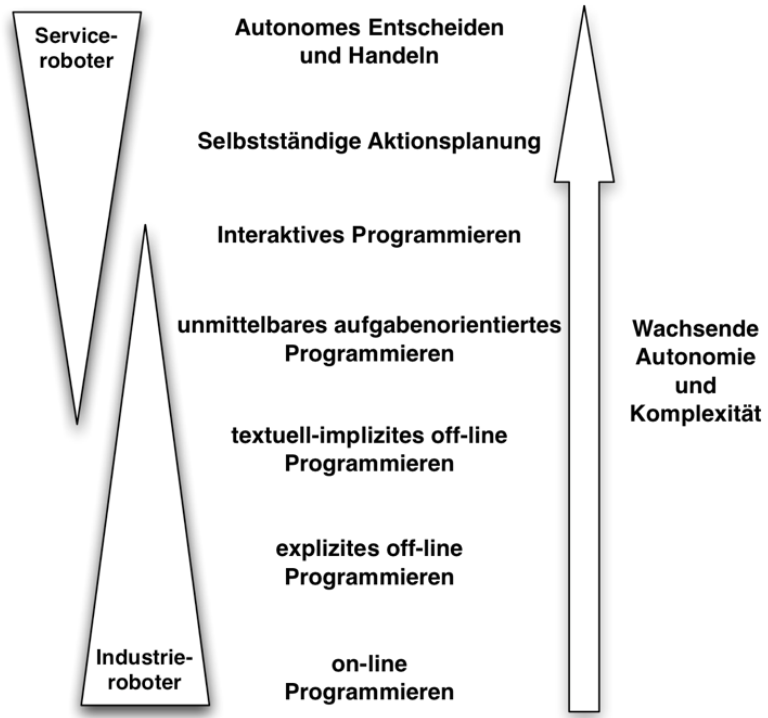
\includegraphics[width=0.5\linewidth]{figures/ch01_ueberblick.png}
\caption{Überblick}
\label{fig:ch01_komp}
\end{figure}
Kriterien:
\begin{itemize}
\item[1.] \textbf{Programmierort:} On-line (prozessnah, am Roboter) vs. Off-line (prozessfern, ohne Roboter)
\item[2.] \textbf{Art der Programmierung:} Direkte vs. indirekte (textuelle oder graphische/gemischte) Programmierung, hybride Verfahren
\item[3.] \textbf{Abstraktionsgrad der Programmierung:} Explizite/bewegungs- bzw. roboterorientierte vs. implizite/aufgabenorientierte Programmierung
\end{itemize}
\begin{figure}[ht]\centering 
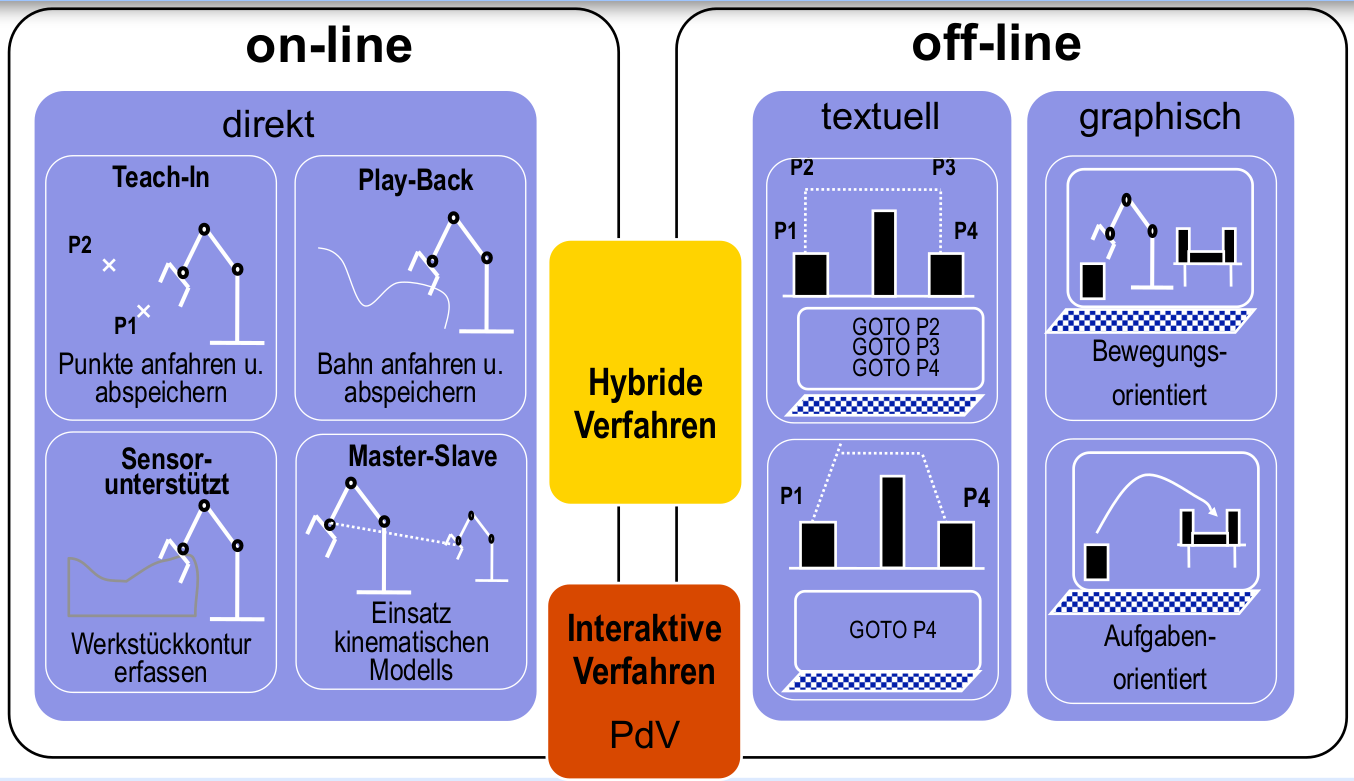
\includegraphics[width=\linewidth]{figures/ch01_schema.png}
\caption{Schema}
\label{fig:ch01_schema}
\end{figure}
\subsection{Arten der Programmierung}
\subsubsection{Direkte/Prozessnahe Programmierung}
\begin{itemize}
\item \textbf{Einstellen des Roboters:} Ältestes Programmierverfahren.
Der Bewegungsbereich jedes Gelenks wird durch Stopper eingeschränkt.
Die Bewegungen erfolgen für jedes Gelenk einzeln bis zum Anschlag.
Zuordnung zwischen Anfahrpunkten zu Stopper kann mit Codiermatritzen erfolgen.
(sogenannter \glqq Bang-Bang-Robot\grqq)\\
Nachteil: sehr kleine Menge von Anfahrpunkten.
\item \textbf{Teach-In Programmierung:} Anfahren markanter Punkte der Bahn mit manueller Steuerung
(Teach Box, Teach Panel, weitere: Spacemouse, Teach-Kugel)\\
Funktionalität einer Teach Box:
\begin{itemize}
\item Einzelbewegung der Gelenke
\item Bewegung des Effektors in 6 Freiheitsgraden
\item Punkte anfahren u. abspeichern
\item Speichern / Löschen von Anfahrpunkten
\item Eingabe von Geschwindigkeiten
\item Eingabe von Befehlen zur Bedienung des Greifers
\item Starten / Stoppen ganzer Programme
\end{itemize}
Vorgehensweise beim Teach-In:
\begin{itemize}
\item Anfahren markanter Punkte der Bahn (= Folge von Zwischenpunkten)
\item Speichern der Gelenkwerte
\item Ergänzung der gespeicherten Werte
um Parameter wie Geschwindigkeit, Beschleunigung usw.
\item Anwendung: in der Fertigungsindustrie (Punktschweißen, Nieten), Handhabungsaufgaben (Pakete vom Fließband nehmen)
\end{itemize}
\item \textbf{Play-Back- (manuelle) Programmierung:}
\begin{itemize}
\item Einstellung des Roboters auf Zero-Force-Control
(Roboter kann durch den Bediener bewegt werden)
\item Abfahren der gewünschten Bahn
\item Speichern der Gelenkwerte: automatisch (definierte Abtastfrequenz) oder manuell (durch Tastendruck)
\item Anwendung: mathematisch schwer beschreibbare Bewegungsabläufe, Integrierung der handwerklichen Erfahrung, typischerweise für Lackieren oder Kleben eingesetzt
\end{itemize}
\begin{table}[hbt]
\centering
\begin{tabular}{|p{13cm}|}
\hline
Nachteile\\
\hline
\vspace{-5mm}
\begin{itemize}
\setlength\itemsep{0em}
\item[-] schwere Roboter schwierig zu bewegen
\item[-] wenig Platz in engen Fertigungszellen für Bediener, dadurch Sicherheitsrisiko
\item[-] hoher Speicherbedarf (bei hoher Abtastrate)
\item[-] schlechte Korrekturmöglichkeiten
\end{itemize}\\
\hline
\end{tabular}
\caption{Nachteile der Play-Back-Programmierung}
\label{tab:PBprog}
\end{table}
\newpage
\item \textbf{Master-Slave-Programmierung:}
\begin{itemize}
\item Bediener führt einen kleinen, leicht bewegbaren Master
Roboter (entspricht einem kinematischen Modell des
Slave-Roboters)
\item Bewegung wird auf den Slave-Roboter übertragen
\item Bewegungen werden synchron ausgeführt
\item Slave-Roboter wirkt als Kraftverstärker
\item Anwendung: Handhabung großer Lasten bzw. großer Roboter
\end{itemize}
\begin{table}[hbt]
\centering
\begin{tabular}{|p{6.5cm}|p{6.5cm}|}
\hline
Vorteile & Nachteile\\
\hline
\vspace{-5mm}
\begin{itemize}
\setlength\itemsep{0em}
\item[+] Möglichkeit, auch schwerste Roboter zu programmieren
\end{itemize}
 &
 \vspace{-5mm}
\begin{itemize}
\setlength\itemsep{0em}
\item[-] teuer, da zwei Roboter benötigt werden
\end{itemize}\\
\hline
\end{tabular}
\caption{Zusammenfassung Master-Slave-Programmierung}
\label{tab:MSprog}
\end{table}
\item \textbf{Sensorunterstützte Programmierung:}\\
Manuell
\begin{itemize}
\item Bediener führt Programmiergriffel (Leuchtstift, Laserstift) entlang der
abzufahrenden Bahn
\item Erfassung der Bewegung durch externe Sensoren (zB. Kameras,
Laserscanner)
\item Berechnung der inversen Kinematik
\end{itemize}
Automatisch
\begin{itemize}
\item Vorgabe des Start- und Zielpunktes
\item Sensorische Ertastung der Sollkontur (zB. über Kraft-Momenten-Sensor)
\end{itemize}
Anwendung: Abspeichern der Bahn als Folge der Gelenkwinkel
Schleifen, Entgraten von Werkstücken	
\end{itemize}
\begin{table}[hbt]
\centering
\begin{tabular}{|p{7.5cm}|p{7.5cm}|}
\hline
Vorteile & Nachteile\\
\hline
\vspace{-5mm}
\begin{itemize}
\setlength\itemsep{0em}
\item[+] schnell bei einfachen Trajektorien
\item[+] sofort anwendbar
\item[+] geringe Fehleranfälligkeit
\item[+] Bediener benötigt keine Programmierkenntnisse
\item[+] kein Modell der Umwelt erforderlich
\end{itemize}
 &
 \vspace{-5mm}
\begin{itemize}
\setlength\itemsep{0em}
\item[-] hoher Aufwand bei komplexen Trajektorien
\item[-] nur mit und am Roboter möglich
\item[-] spezifisch für einen Robotertyp
\item[-] Verletzungsgefahr durch Roboter
\end{itemize}\\
\hline
\end{tabular}
\caption{Zusammenfassung Direkte Programmierung}
\label{tab:dirprog}
\end{table}
\subsubsection{Textuelle Verfahren}
Erstellung von Robotersteuerprogrammen erfolgt mittels erweiterter,
höherer Programmiersprachen (PasRo, Val, etc.)
\\ \\
\textbf{Sprache:} (DIN 66025)
\begin{itemize}
\item Programm = Menge numerierter Sätze\\
z.B. \glqq N70 G00 X20 Z12\grqq{} entspricht Werkzeug im Eilgang (G00) an Position X=20 Z=12 bewegen. (N = Satznummer)
\item Sprachen:
\begin{itemize}
\item APT (Automatically Programmed Tools), 1961 MIT
\item EXAPT (Extended Subset of APT), 1966 Aachen
\end{itemize}
\end{itemize}

\begin{table}[!h]
\centering
\begin{tabular}{|p{7.5cm}|p{7.5cm}|}
\hline
Vorteile & Nachteile\\
\hline
\vspace{-5mm}
\begin{itemize}
\setlength\itemsep{0em}
\item[+] Programmierung kann unabhängig vom Roboter erfolgen
\item[+] strukturierte, übersichtliche Programmierlogik
\item[+] Erstellung komplexer Programme (Einbezug von Wissensbasis,
Weltmodell, Auswertung von Sensoren)
\end{itemize}
 &
 \vspace{-5mm}
\begin{itemize}
\setlength\itemsep{0em}
\item[-] Bediener benötigt Programmierkenntnisse
\item[-] keine / schlechte Korrekturmöglichkeiten
\end{itemize}\\
\hline
\end{tabular}
\caption{Zusammenfassung Textuelle Verfahren}
\label{tab:textprog}
\end{table}
\subsubsection{Graphische/Gemischte Verfahren}
\begin{itemize}
\item Graphische Darstellung von Kontrollstrukturen (if/else, Schleifen,
Marken...)
\item Kopplung mit Visualisierungs-Tool und Simulations-Tool (z.B. RobCAD)
\item  Trajektorien durch Interpolation aus Stützpunkten, Freihandzeichnen,
analytisch
\item Operationen Icon- oder Menu-gesteuert
\item Simple graphische Programmierung, z.B. Lego Mindstorms:
Leicht verständliche, ikonische Programmierung aber beschränkte Möglichkeiten
\item Graphische Programmierung basierend auf sensorieller Erfassung der
Benutzervorführung:\\ Simulation der Roboterprogramme
\end{itemize}
\begin{table}[hbt]
\centering
\begin{tabular}{|p{7.5cm}|p{7.5cm}|}
\hline
Vorteile & Nachteile\\
\hline
\vspace{-5mm}
\begin{itemize}
\setlength\itemsep{0em}
\item[+] Programmierer benötigt weniger Programmierkenntnisse
\item[+] einfache Programmierung, leichte Fehlererkennung
\item[+] schnelles Erstellen komplexer Programme (rapid prototyping)
\end{itemize}
 &
 \vspace{-5mm}
\begin{itemize}
\setlength\itemsep{0em}
\item[-] sensorielle Benutzererfassung noch zu ungenau
\item[-] Leistungsfähige Hardware für Signalanalyse, Modellierung, ...
\item[-] Komplexe Modelle benötigt
\item[-] 2D-Sicht des Anwenders
\end{itemize}\\
\hline
\end{tabular}
\caption{Zusammenfassung Graphische Verfahren}
\label{tab:textprog}
\end{table}
\newpage
\subsection{Abstraktionsgrad der Programmierung}
\subsubsection{Explizite/Roboterorientierte Programmierung}
\textcolor{red}{\glqq Wie ist es zu tun?\grqq} \\
Bewegungen und Greiferbefehle sind direkt in eine Programmiersprache eingebunden.\\
Das Aufgabenmodell ist gegeben durch Anfangs- und Endzustand (z.B. Relationale Darstellung). Ein Beispiel ist in \autoref{cranfield} dargestellt.\\
\begin{figure}[h!]\centering 
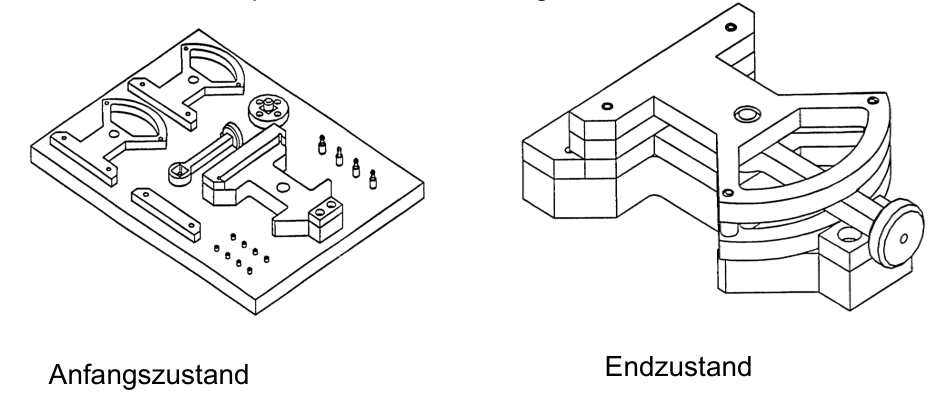
\includegraphics[width=0.7\linewidth]{figures/ch01_cranfield.png}
\caption{Der Cranfield-Montage-Benchmark}
\label{cranfield}
\end{figure}\\
\paragraph{Anwender $\rightarrow$ Roboter}
Jedes Robotersystem besitzt eine roboterabhängige Steuerungsebene, welche folgende Eigenschaften kapselt:
\begin{itemize}
\item Ansteuerung der Hardware (sowohl interne als auch externe)
\item Bewegungsaktionen
\item Lokale Modelle
\item Elementare Operationen (erfordern evtl. Echtzeitregelung)
\end{itemize}
\begin{figure}[h!]\centering 
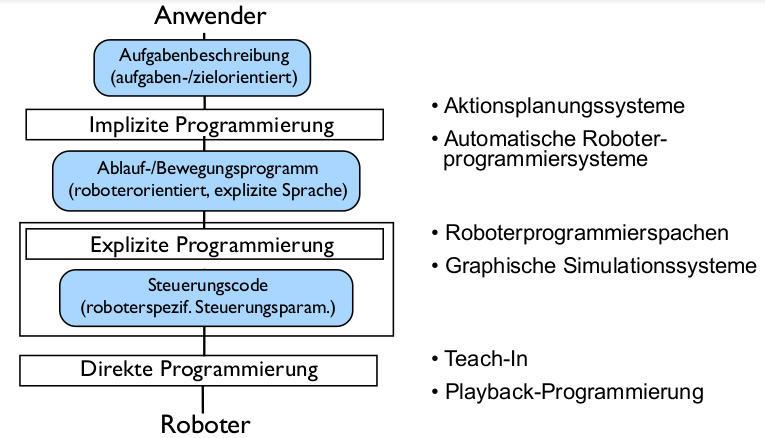
\includegraphics[width=0.7\linewidth]{figures/ch01_einordnung.png}
\caption{Einordnung roboterorientierte Programmierung}
\label{einord}
\end{figure}
\paragraph{Anforderungen an die roboterorientierte Programmierung}
\begin{itemize}
\item Positions-, Geschwindigkeitsregelung der aktiven Komponenten (z.B. Gelenke, Räder)
\item Auslesen und Parametrieren der internen und externen Sensorik
\item Koordinatentransformationen, direkte und inverse Kinematik
\item Sensorabhängige Regelung
\item Verfahren auf Trajektorien
\item Generierung und Zusammensetzen von Trajektorien zu komplexen Bewegungen
\item Verkettung komplexer Bewegungen zu Elementaroperationen
\end{itemize}
\paragraph{Komponenten der roboterorientierten Programmierung}
\autoref{zykl}\\
\begin{figure}[h!]\centering 
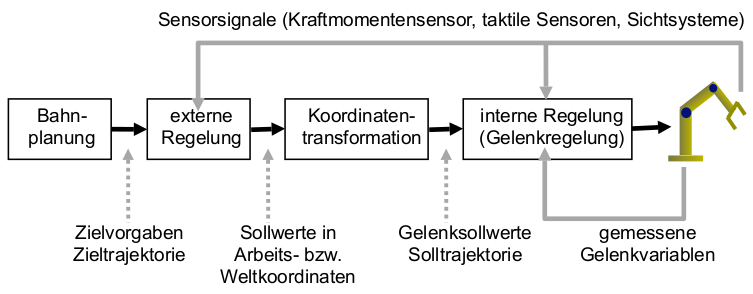
\includegraphics[width=0.7\linewidth]{figures/ch01_zykl.png}
\caption{Regelungszyklus eines Roboters}
\label{zykl}
\end{figure}\\
\paragraph{Sprachelemente von Roboterprogrammiersprachen}
\begin{itemize}
\item Befehle für:
\begin{itemize}
\item Bewegung eines oder mehrerer Roboter
\item Betrieb von Greifern / Werkzeugen
\item Ein-/Ausgabe von Daten / Signalen über Schnittstellen
\item Externe Sensoren
\item Zur Synchronisation / Kommunikation zwischen Prozessen
\item Parallelverarbeitung
\item Zur logischen Verkettung von Koordinatensystemen
\end{itemize}
\item Anweisungen zur Ablaufsteuerung
\item Definition generischer Operationen (zB. Armbewegung + Griff $\rightarrow$ ein Operator)
\end{itemize}
\paragraph{Bewegungsanweisungen}
\begin{itemize}
\item Bewegungen im Gelenkwinkelraum:
\begin{itemize}
\item Bewege alle Gelenke mit max. Geschwindigkeit
\item Regelung der Geschwindigkeiten mit gleichzeitiger Beendigung der Bewegung aller Gelenke
\end{itemize}
\item Kartesische Bewegungen (Stellung des TCPs)
\begin{itemize}
\item Erfordert inverse Kinematik
\item Nutzung von Frames, z.B. relativ zu einem Objekt
\end{itemize}
\item Geometriebezogene Bahndefinition
\end{itemize}
\begin{table}[hbt]
\centering
\begin{tabular}{|p{7.5cm}|p{7.5cm}|}
\hline
Vorteile & Nachteile\\
\hline
\vspace{-5mm}
\begin{itemize}
\setlength\itemsep{0em}
\item[+] Hohe Einstellgenauigkeit der Position
\item[+] Hohe Wiederholgenauigkeit
\item[+] eindeutige Roboterkonfiguration
\item[+] keine inverse Kinematik erforderlich
\end{itemize}
 &
 \vspace{-5mm}
\begin{itemize}
\setlength\itemsep{0em}
\item[-] Abhängigkeit von Robotertyp
\item[-] kein Bezug der Gelenkwinkel zur Objektlage
\end{itemize}\\
\hline
\end{tabular}
\caption{Bewegungen im Gelenkwinkelraum}
\label{tab:bew}
\end{table}
\paragraph{Sprachelemente -- Semantik von Greiferbefehlen}
\begin{itemize}
\item Verschiedene Greifertypen: evtl. mit taktiler und/oder Kraftsensorik
\item Backengreifer: Industrie, Forschung (z.B. 3-Finger-Hand)
\end{itemize}
Mit zunehmender Abstraktion:
\begin{enumerate}
\item Steuerung im Gelenkwinkel-Raum
\begin{itemize}
\item Anzahl der Freiheitsgrade bestimmt Anzahl der Parameter (Backengreifer: 1, menschl. Hand: 22)
\item Wenig Kapselungs-Aufwand (keine inverse Kinematik nötig) 
\item Hand-abhängig
\item Kein Bezug zwischen Fingerstellung und Handstellung
\end{itemize}
\item Steuerung im kartesischen/ zylindrischen/... Raum
\begin{itemize}
\item Parameter: Position/Orientierung jedes Fingers/ jeder Fingerspitze
\item Inverse Kinematik nötig
\item Berechnung aus Greif-/ Bewegungsplanung oder aus menschlicher Vorführung
\item Mögliche Konfigurationen (Konfigurationsraum) handabhängig
\end{itemize}
\item Semantische Steuerung
\begin{itemize}
\item Parameter: Griff-Form, zu greifendes Objekt, Objektgröße, Objektform, ...
\item Mapping auf Roboterhand nötig
\item Übertragbar auf andere Roboterhände (mögliche Griffe handabhängig)
\item Griff-Form vom Menschen lernbar
\end{itemize}
\end{enumerate}
\paragraph{Zusammenfassung -- Explizite Programmierung} Nur in Verbindung mit (abstrakten) Programmiersprachen
\begin{table}[hbt]
\centering
\begin{tabular}{|p{7.5cm}|p{7.5cm}|}
\hline
Vorteile & Nachteile\\
\hline
\vspace{-5mm}
\begin{itemize}
\setlength\itemsep{0em}
\item[+] beliebig komplexe Bahnen
\item[+] Anbindung von Sensoren
\item[+] reaktive Planung
\end{itemize}
 &
 \vspace{-5mm}
\begin{itemize}
\setlength\itemsep{0em}
\item[-] Keine standardisierte Programmiersprache
\item[-] Kenntnis der Programmiersprache
\end{itemize}\\
\hline
\end{tabular}
\caption{Bewegungen im Gelenkwinkelraum}
\label{tab:bew}
\end{table}
\subsubsection{Implizite/Aufgabenorientierte Programmierung}
\textcolor{red}{\glqq Was ist zu tun?\grqq} \\
Die Aufgabe, die der Roboter durchführen soll, wird beschrieben, z.B. in Form von Zuständen.
\begin{itemize}
\item Abstrakte Form der Programmierung erfolgt in den Phasen\\
1. Modellierung der Umwelt\\
2. Spezifikation der Aufgaben\\
3. Erzeugung der Roboterprogramme
\item u. U. erfolgt vor der Ausführung eine Überprüfung des
Roboterprogramms (Simulation)
\item Beispiel: Einschenken unter Berücksichtigung von Hindernissen
\item Details im kommenden Kapitel
\end{itemize}

\section{Aufgabenorientierte Programmierung} %(2. VL)
\subsection{Umweltmodellierung}
\begin{figure}[ht]\centering 
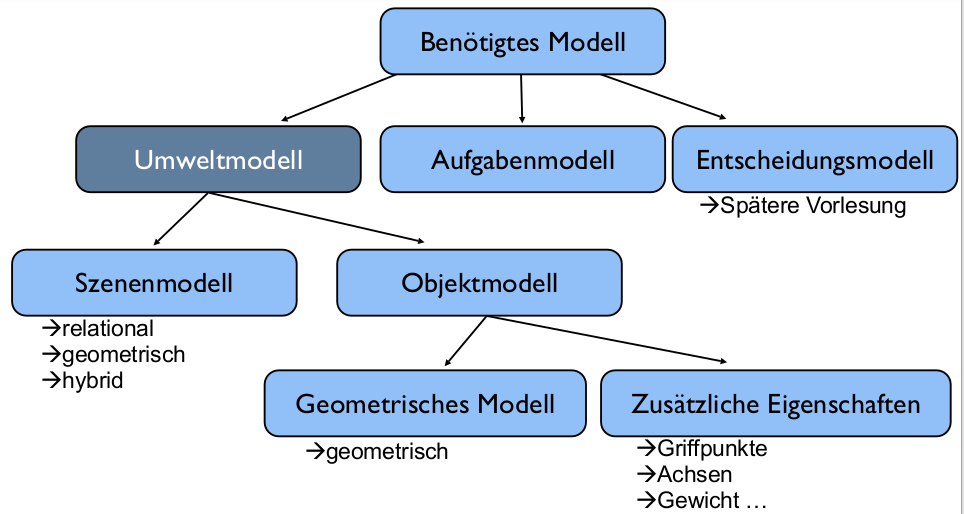
\includegraphics[width=0.6\linewidth]{figures/ch02_umweltmodell.png}
\caption{Umweltmodell}
\label{fig:ch02_um}
\end{figure}

%Keine Umlaute in labels!!!
\subsubsection{Objektmodell}
Die geometrische Beschreibung von Objekten beinhaltet:
\begin{itemize}
\setlength\itemsep{0em}
\item graphische Darstellung
\item Kollisionsberechnungen, Kontaktberechnung in Griffplanung, ...
\item physikalisch-dynamische Simulation der Effekte von Handlungen auf die Umwelt
\item geometriebezogene Bewegungsplanung
\end{itemize}
Es gibt drei Ansätze zur geometrischen Modellierung (\autoref{fig:obrepr}): 
\begin{enumerate}
\item Kantenmodelle
\item Flächenmodelle
\item Volumenmodelle
\end{enumerate}
\begin{figure}[h!]
	\centering
	\begin{subfigure}{.25\textwidth}
		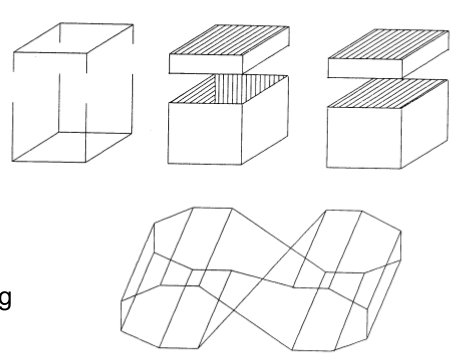
\includegraphics[width=\textwidth]{figures/ch02_kanten.png}
		\caption{}
	\end{subfigure}
	\begin{subfigure}{.25\textwidth}
		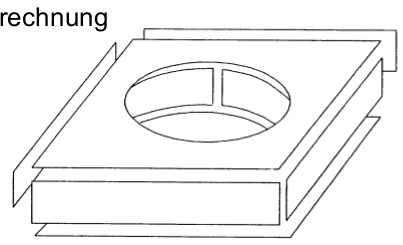
\includegraphics[width=\textwidth]{figures/ch02_flaechen.png}
		\caption{}
	\end{subfigure}
	\begin{subfigure}{.25\textwidth}
		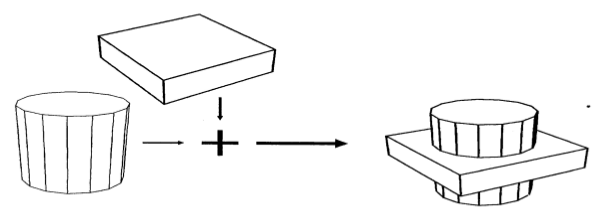
\includegraphics[width=\textwidth]{figures/ch02_volumen.png}
		\caption{}
	\end{subfigure}
	\caption{Objektrepr\"{a}entation}
	\label{fig:obrepr}
\end{figure}
\paragraph*{Kanten}
Nur die Kanten werden gespeichert, d.h. Punkte und Verbindungen (Gerade, Polygonzug, Bezierkurve, ... ).
\begin{table}[hbt]
\centering
\begin{tabular}{|p{6.5cm}|p{6.5cm}|}
\hline
Vorteile & Nachteile\\
\hline
\vspace{-5mm}
\begin{itemize}
\setlength\itemsep{0em}
\item[+] einfache Daten
\item[+] wenige Daten
\end{itemize}
 &
 \vspace{-5mm}
\begin{itemize}
\setlength\itemsep{0em}
\item[-] Mehrdeutigkeiten
\item[-] hoher Eingabeaufwand
\item[-] keine Kollisionsberechnung
\item[-] kein Schnitt
\end{itemize}\\
\hline
\end{tabular}
\caption{Zusammenfassung -- Kantenmodelle}
\label{tab:Kantenmod}
\end{table}\\ 
\paragraph*{Flächen}
Flächen können exakt modelliert werden, wenn sie \textcolor{red}{analytisch gegeben} sind (eine 3D Kugel beispielsweise durch $r = ||x-p||$, wobei $r$ der Radius und $p$ der Mittelpunkt ist).
\begin{table}[hbt]
\centering
\begin{tabular}{|p{6.5cm}|p{6.5cm}|}
\hline
Vorteile & Nachteile\\
\hline
\vspace{-5mm}
\begin{itemize}
\setlength\itemsep{0em}
\item[+] Geschlossene Darstellung (wenig Speicherbedarf)
\item[+] Analytische Darstellung erlaubt einfache Rechenverfahren (z.B.
Schnitt von Ebenen / Kugeln $\rightarrow$ schnelle Kollisionsberechnung)
\end{itemize}
 &
 \vspace{-5mm}
\begin{itemize}
\setlength\itemsep{0em}
\item[-] Wenige Flächen sind analytisch darstellbar
\end{itemize}\\
\hline
\end{tabular}
\caption{Flächen -- analytisch}
\label{tab:Flaechen-analyt}
\end{table}\\ 
Ansonsten werden sie \textcolor{red}{approximativ} durch Bildung einer großen Fläche aus einem Netz (\glqq Mesh\grqq ) von einfachen Einzelflächen (z.B. Dreiecke, Vierecke) modelliert.\\
\begin{table}[hbt]
\centering
\begin{tabular}{|p{6.5cm}|p{6.5cm}|}
\hline
Vorteile & Nachteile\\
\hline
\vspace{-5mm}
\begin{itemize}
\setlength\itemsep{0em}
\item[+] Definition sehr einfach
\item[+] einfache Algorithmen
\end{itemize}
 &
 \vspace{-5mm}
\begin{itemize}
\setlength\itemsep{0em}
\item[-] hoher Speicherbedarf
\item[-] hoher Rechenaufwand
\end{itemize}\\
\hline
\end{tabular}
\caption{Flächen -- approximativ}
\label{tab:Flaechen_approx}
\end{table}
\newpage
Hierbei werden Freiformflächen im einfachsten Fall durch \textbf{Dreiecksflächen} approximiert:
\begin{itemize}
\item[] Gegeben seien 3 Punkte im Raum $P_1 , P_2 , P_3$.
\item[] Damit hat die Fläche folgende Gleichung: $F(u,v)=u\cdot P_1 +v\cdot P_2 +(1-u-v)\cdot P_3$ mit $0 \leq u,v, u+v \leq 1$.
\begin{center}
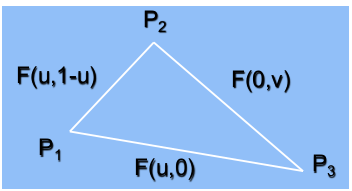
\includegraphics[width=.3\linewidth]{figures/ch02_dreieck.png}
\end{center}
\end{itemize}
Oder sie werden durch \textbf{Bilineare Viereckselemente / Pflaster} approximiert:
\begin{itemize}
\item[] Gegeben sind 4 Punkte im Raum $P_1 , P_2 , P_3, P_4$
\item[] Damit wird die Fläche definiert durch $F(u,v)=(1-u)(1-v) \cdot P_1 + (1-u)v \cdot P_2 + u(1-v) \cdot P_3 + uv \cdot P_4$ mit $0 \leq u \leq 1, 0 \leq v \leq 1$. 
\begin{center}
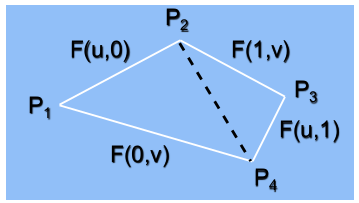
\includegraphics[width=.3\linewidth]{figures/ch02_pflaster.png}
\end{center}
\end{itemize}
\begin{table}[hbt]
\centering
\begin{tabular}{|p{6.5cm}|p{6.5cm}|}
\hline
Vorteile & Nachteile\\
\hline
\vspace{-5mm}
\begin{itemize}
\setlength\itemsep{0em}
\item[+] Flächenelemente können gekrümmt sein
$\rightarrow$ weniger Gitterpunkte bei gleich guter Approximation
\end{itemize}
 &
 \vspace{-5mm}
\begin{itemize}
\setlength\itemsep{0em}
\item[-] Rechnen mit gekrümmten Flächen ist aufwendig
\end{itemize}\\
\hline
\end{tabular}
\caption{Approximation durch Vierecke}
\label{tab:Viereck_approx}
\end{table}
Zudem können Flächen durch \textbf{Bezierflächen}, einer Erweiterung der Bezierkurven beschrieben werden:
\begin{itemize}
\item[] Gegeben ist ein Gitter von Führungspunkten $P_{ij}, 0 \leq i \leq N$ und $0 \leq j \leq M$.
\item[] Damit ist die Fläche beschrieben durch $F(u,v) = \sum_{i=0}^N \sum_{j=0}^M P_{ij} \cdot B_{i,N}(u) \cdot B_{j,M}(v)$\\
 mit $B_{i,N}(u) = (1-u)B_{i,N-1}(u)+uB_{i-1,N-1}(u)$\\
 und $B_{j,M}(v) = (1-v)B_{j,M-1}(v)+vB_{j-1,M-1}(v)$.
\item[] Die $B_{i,N}$ bzw. $B_{j,M}$ heißen auch Bernsteinpolynome.
\begin{center}
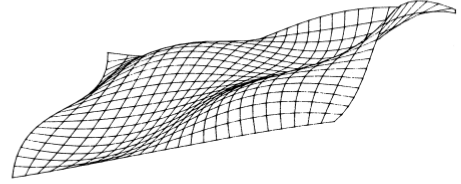
\includegraphics[width=.4\linewidth]{figures/ch02_bezier.png}
\end{center}
\end{itemize}
\begin{table}[hbt]
\centering
\begin{tabular}{|p{6.5cm}|p{6.5cm}|}
\hline
Vorteile & Nachteile\\
\hline
\vspace{-5mm}
\begin{itemize}
\setlength\itemsep{0em}
\item[+] effiziente Verfahren 
\item[+] entspricht dem Vorgehen während der Modellierung
\item[+] schnelle Kollisions- und Abstandsberechnung
\end{itemize}
 &
 \vspace{-5mm}
\begin{itemize}
\setlength\itemsep{0em}
\item[-] hoher Eingabeaufwand
\item[-] Darstellung aufwendig
\item[-] Problem bei Schnittoperationen
\item[-] Inkonsistenzen möglich
\end{itemize}\\
\hline
\end{tabular}
\caption{Zusammenfassung -- Flächenmodelle}
\label{tab:Flaechenmod}
\end{table}
\noindent
\paragraph*{Volumen} Vier verschiedene Arten von Volumenmodellen:\\ \\
\textbf{Parametrische Modelle}:\\
Grundkörper und topologische Operationen auf diesen (Schnitt, Vereinigung, ... ) werden abgespeichert. 
\begin{table}[hbt]
\centering
\begin{tabular}{|p{6.5cm}|p{6.5cm}|}
\hline
Vorteile & Nachteile\\
\hline
\vspace{-5mm}
\begin{itemize}
\setlength\itemsep{0em}
\item[+] eindeutige Objektbeschreibung 
\item[+] geringer Eingabeaufwand 
\item[+] Ergebnis von Operationen sind korrekte Objekte
\end{itemize}
 &
 \vspace{-5mm}
\begin{itemize}
\setlength\itemsep{0em}
\item[-] hoher Implementierungsaufwand
\item[-] Einbindung von Freiformflächen schwierig
\end{itemize}\\
\hline
\end{tabular}
\caption{Volumenmodelle -- parametrisch}
\label{tab:Volmod}
\end{table}\\ 
Die Objekte sind bereits vorhanden und können durch Angabe von Parametern angepaßt werden (Varianten).\\
Konsistenzprüfungen sind notwendig (\autoref{fig:kons})! \\
\begin{figure}[h!]
	\centering 
	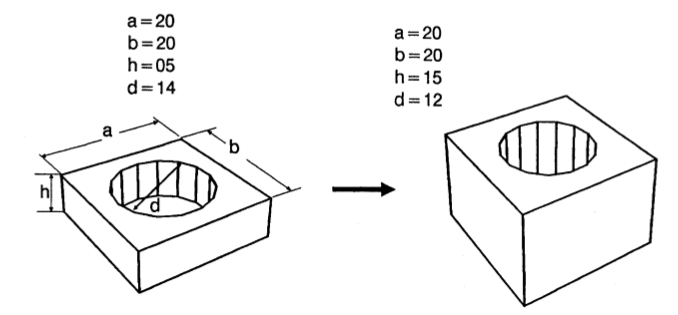
\includegraphics[width=0.3\linewidth]{figures/ch02_kons.png}
	\caption{Konsistenzprüfung: $d < min(a,b)$}
\label{fig:kons}
\end{figure}\\
\noindent
\textbf{Zellenzerlegung}:\\
 Objekte werden aus disjunkten Elementarzellen aufgebaut. Verwendung finden einfache geometrische Objekte z,B. Tetraeder, Quader, ...
Benutzt in der Strukturanalyse mit Finite-Elemente-Methoden (FEM).
\newpage
Diese Modelle können auf drei Arten umgesetzt werden:
\begin{enumerate}
\item Boundary Repräsentation
\item Constructive Solid Geometry (CSG)
\item Zellenbelegung
\end{enumerate}
\textbf{Boundary Repräsentation}: Hierarchische Darstellung eines Objektes durch begrenzende
Elemente, i.d.R. Kanten oder Flächen. \autoref{fig:brep} zeigt ein Beispiel.\\
\begin{figure}[h!]
	\centering 
	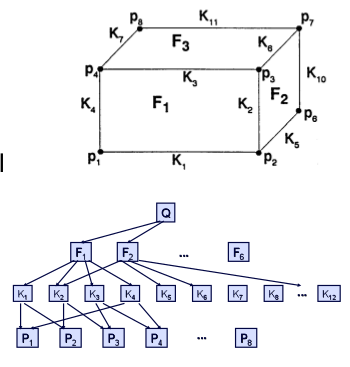
\includegraphics[width=0.3\linewidth]{figures/ch02_brep.png}
	\caption{Elemente eines Quaders im Flächenmodell: Quader $Q$, Flächen $F_i : i \in \{1,...,6\}$, Kanten $K_i : i \in \{1,...,12\}$, Ecken $P_i : i \in \{1,...,8\}$}
\label{fig:brep}
\end{figure}
Vorteile: aus der topologischen Struktur Information über z.B.:
\begin{itemize}
\item Welche Flächen gehören zum Objekt?
\item Welche Kanten gehören zur Fläche? $\rightarrow$ kantenbasierte Objekterkennung
\item Zu welchem Objekt gehört eine Fläche?
\item Zu welchem Objekt gehört eine Kante?
\item Welche Flächen stoßen aneinander?
\end{itemize}
\noindent
\textbf{Constructive Solid Geometry (CSG)}:
Es gibt eine Menge von einfachen Grundkörpern, die parametriert
werden können (\autoref{fig:csg}). 
\begin{figure}[h!]
	\centering
	\begin{subfigure}{.7\textwidth}
		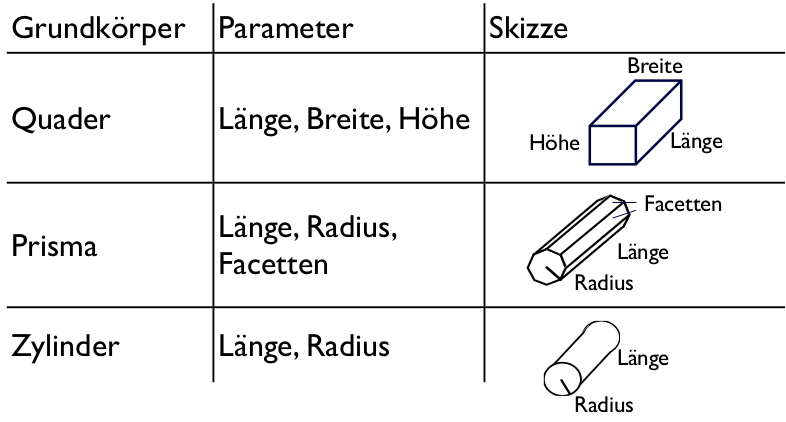
\includegraphics[width=\textwidth]{figures/ch02_csg.png}
	\end{subfigure}
	\begin{subfigure}{.7\textwidth}
		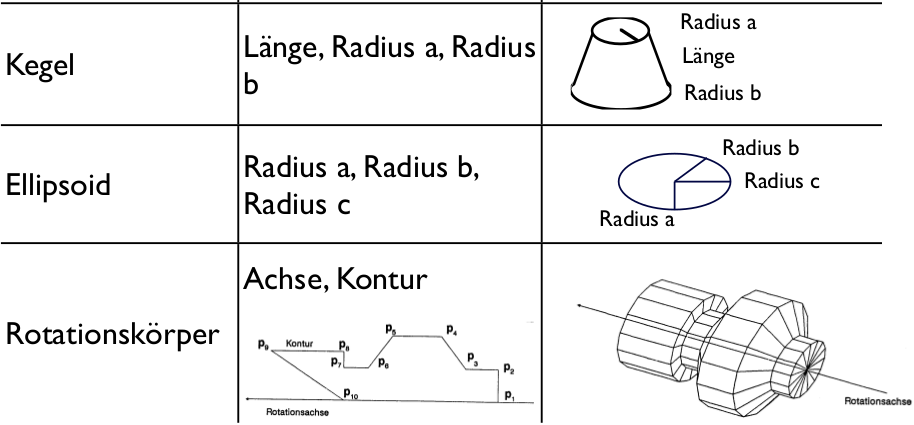
\includegraphics[width=\textwidth]{figures/ch02_csg1.png}
	\end{subfigure}
	\caption{Constructive Solid Geometry}
	\label{fig:csg}
\end{figure}
Auf ihnen sind verschiedene Operationen definiert, z.B.
\begin{table}[!hb]
\centering
\begin{tabular}{|p{6.5cm}|p{6.5cm}|}
\hline
Objekt $A$ 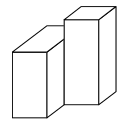
\includegraphics[width=.07\textwidth]{figures/ch02_a.png} & Objekt $B$ 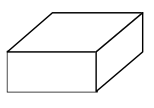
\includegraphics[width=.07\textwidth]{figures/ch02_b.png}\\
\hline
Vereinigung $A \cup B$ (Summe) & 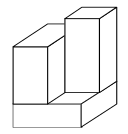
\includegraphics[width=.07\textwidth]{figures/ch02_ab.png}\\
\hline
Schnitt $A \cap B$ & 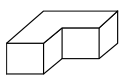
\includegraphics[width=.07\textwidth]{figures/ch02_ab1.png} \\
\hline
Differenz $A / B$ & 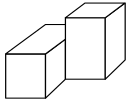
\includegraphics[width=.07\textwidth]{figures/ch02_ab2.png}\\
\hline
Sweep:
Ein Grundelement (u.U. eine Fläche) wird entlang einer Raumkurve
verschoben. Der durchdrungene Raum stellt das neue Objekt dar. & \\
\hline
\end{tabular}
\caption{CSG -- Operatoren}
\label{tab:csg_ops}
\end{table}\\ \\
\textbf{Zellenbelegung}:
Der Raum wird in mehrere Zellen unterteilt (i.d.R. 8 Zellen: \glqq Octree\grqq).
Wenn eine Zelle komplett vom Objekt belegt ist, als \glqq belegt\grqq{} markieren.
Wenn die Zelle nur teilweise belegt ist, dann wird auf diese Zelle das
Verfahren rekursiv angewendet. Ansonsten ist die Zelle leer.
Die Rekursion terminiert bei einer vorbestimmten minimalen Zellgröße.
Teilbelegte kleinste Zellen werden als belegt markiert. Siehe \autoref{zb}.
\begin{figure}[h!]
	\centering
	\begin{subfigure}{.45\textwidth}
		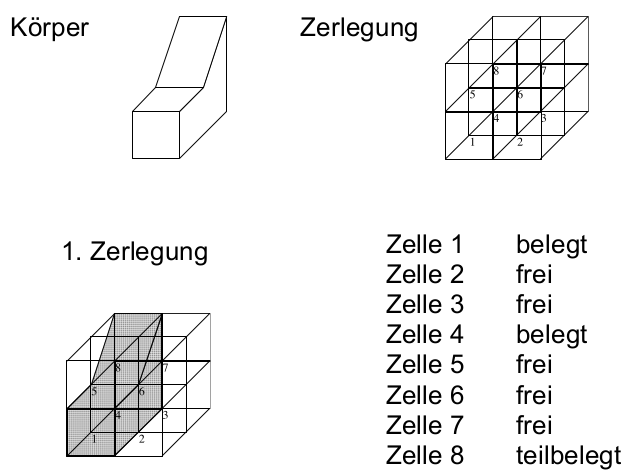
\includegraphics[width=\textwidth]{figures/ch02_zb.png}
	\end{subfigure}
	\begin{subfigure}{.45\textwidth}
		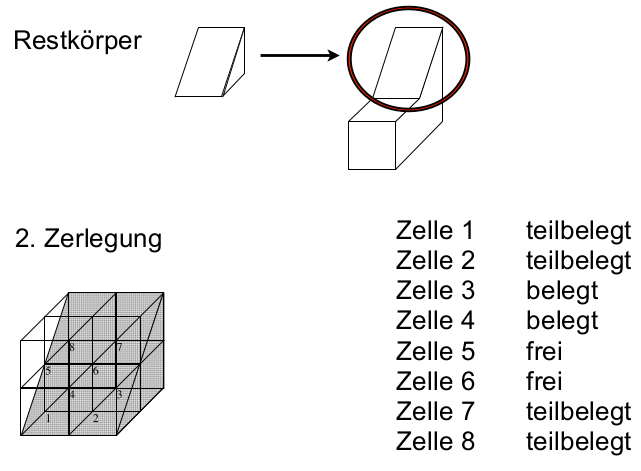
\includegraphics[width=\textwidth]{figures/ch02_zb1.png}
	\end{subfigure}
	\caption{Beispiel -- Zellenbelegung}
	\label{zb}
\end{figure}
\newpage
\subsection{Aufgabenmodellierung}
\begin{figure}[h!]\centering 
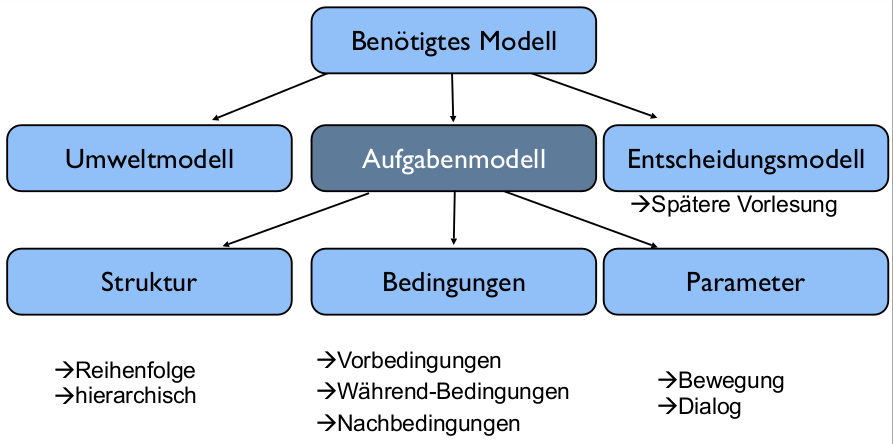
\includegraphics[width=0.6\linewidth]{figures/ch02_aufgabenmodell.png}
\caption{Aufgabenmodell}
\label{fig:ch02_am}
\end{figure}
%kognitive Lücke?
\begin{figure}[ht]\centering 
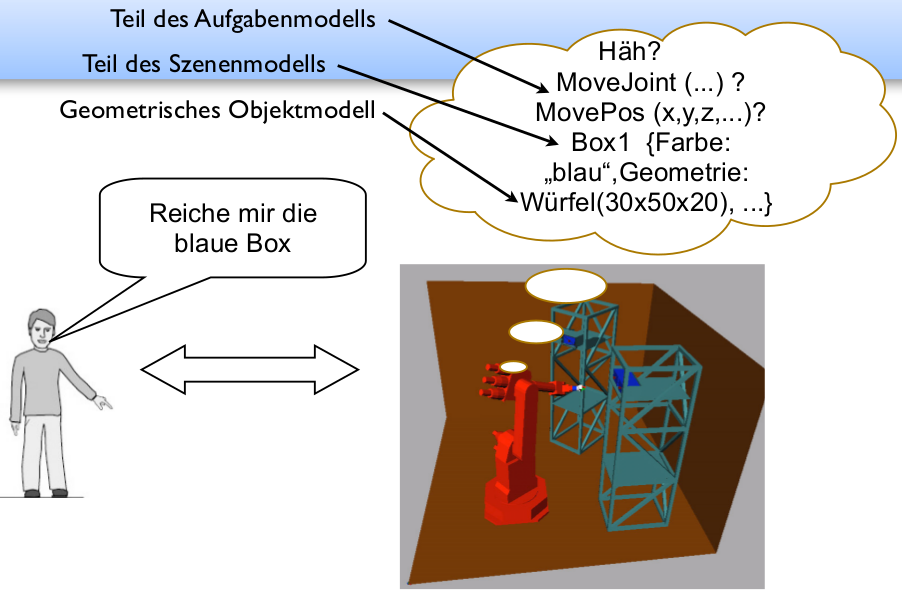
\includegraphics[width=0.6\linewidth]{figures/ch02_beispiel.png}
\caption{Beispiel}
\label{fig:ch02_bsp}
\end{figure}
\begin{figure}[h!]\centering 
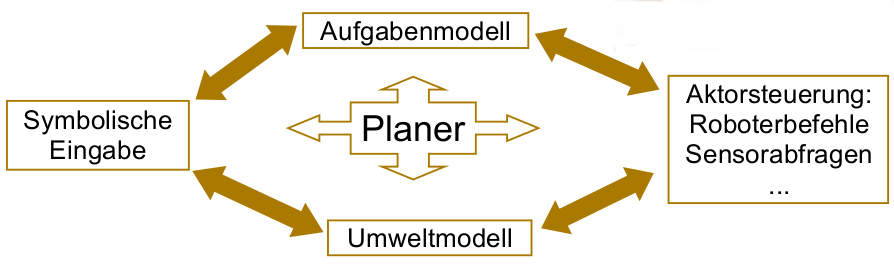
\includegraphics[width=0.6\linewidth]{figures/ch02_planer.png}
\caption{Einordnung des Aufgabenmodells}
\label{fig:ch02_ord}
\end{figure}
\textbf{Anforderungen an das Aufgabenmodell}:
\begin{itemize}
\item Erweiterbarkeit
\item Erklärbarkeit
\item Wiederverwendbarkeit
\item Integration des Wissens in ein Planungssystem
\end{itemize}
\newpage
\paragraph*{Symbolische Abstraktion}
Benutzer beschreibt die Aufgabe mit seinen Worten\\ (z.B. \glqq Bring mir Tee!\grqq) 
\begin{itemize}
\ita Abbildung: Erzeugung der Roboterbefehle über mehrere Stufen (vgl. \autoref{symbab})
\ita \glqq Fahre in die ‚Küche‘, greife ein Glas, fahre zurück und reiche mir den Becher.\grqq
\ita \glqq DriveTo(...), SearchObject(...), MoveArm(...), Grasp(Becher), MoveArm(...), DriveTo(...), MoveArm(...) ...!\grqq
\end{itemize}
\begin{figure}[h!]\centering 
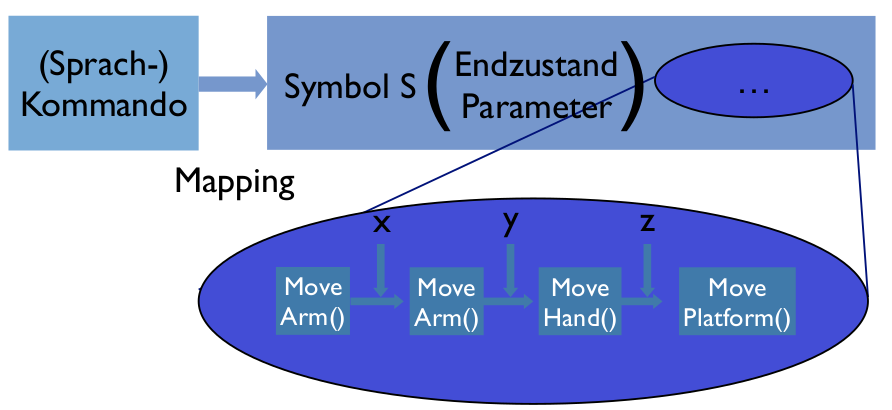
\includegraphics[width=0.6\linewidth]{figures/ch02_symbab.png}
\caption{Symbolische Abstraktion}
\label{symbab}
\end{figure}
\paragraph*{Modellierung der Reihenfolge von Operatoren/Symbolische Handlungsatome}
\begin{itemize}
\item In den gegebenen Beispielen wurden bereits implizit Handlungsatome angenommen
\item Die kleinsten auszuführenden Handlungseinheiten werden als
Elementaroperationen oder atomare Handlungen bezeichnet.
\item Komplexe Handlungen werden aus Elementaroperationen zusammengesetzt. Diese
können dazu üblicherweise parametriert werden.
\item Jeder Roboter besitzt eine endliche Menge an Elementaroperationen.
\end{itemize}
\paragraph*{Drei Ansätze für das Aufgabenmodell}
\begin{enumerate}
\item Sequentiell (\autoref{seq}): Festgelegte Folge von elementaren Aktionen 
\item Vorranggraph (\autoref{vorgra}): Darstellung der Abhängigkeiten
\item Hierarchisch (\autoref{hierar}): Abstraktion von Teilhandlungen
\end{enumerate}
\begin{figure}[h!]
	\centering
	\begin{subfigure}{.25\textwidth}
		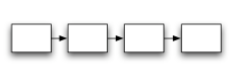
\includegraphics[width=\textwidth]{figures/ch02_ans.png}
		\caption{Sequentiell}
		\label{seq}
	\end{subfigure}
	\begin{subfigure}{.25\textwidth}
		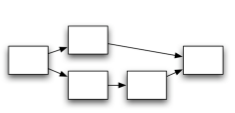
\includegraphics[width=\textwidth]{figures/ch02_ans1.png}
		\caption{Vorranggraph}
		\label{vorgra}
	\end{subfigure}
		\begin{subfigure}{.25\textwidth}
		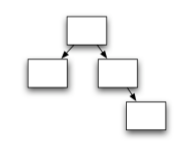
\includegraphics[width=\textwidth]{figures/ch02_ans2.png}
		\caption{Hierarchie}
		\label{hierar}
	\end{subfigure}
	\caption{Ansätze für das Aufgabenmodell}
	\label{ans}
\end{figure}
\newpage
\textbf{Sequentielle Handlungsbeschreibung}:
\begin{itemize}
\item Folge von (parametrierten) atomaren Handlungen
\item Eindeutig festgelegte Reihenfolge
\item Reihenfolge und Anordnung nicht unbedingt erklärbar (lesbar)
\item Bedingungen, Alternativen, etc. schlecht darstellbar
\item Sinnvoll für einfache Aufgaben oder sehr strukturierte Umgebungen (z.B. Leittechnik/Industrie)
\item Komplexe Handlungen: Rein sequentielle Beschreibungen nicht mächtig genug!
\item Ausführung sequentiell beschriebener Handlungen trivial
\item Linearer Handlungsfluss
\item Ausführung besteht aus: Anstoßen einer Elementarhandlung, evtl. Handlungsüberwachung und nach (erfolgreicher) Beendigung Übergang zur nächsten Elementarhandlung
\item Einfache Mechanismen zur Ausführung nötig!
\end{itemize}
\textbf{Vorranggraph}:
\begin{figure}[h!]
	\centering
	\begin{subfigure}{.45\textwidth}
		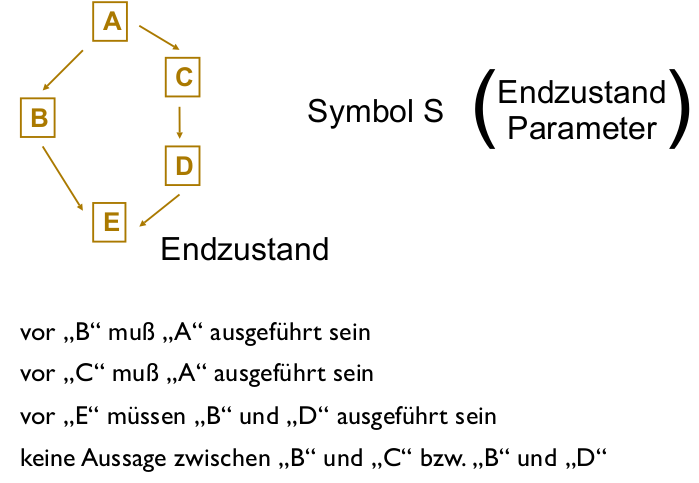
\includegraphics[width=\textwidth]{figures/ch02_vg-mod.png}
		\caption{Modellierung der Reihenfolge: Vorranggraph}
	\end{subfigure}
	\begin{subfigure}{.45\textwidth}
		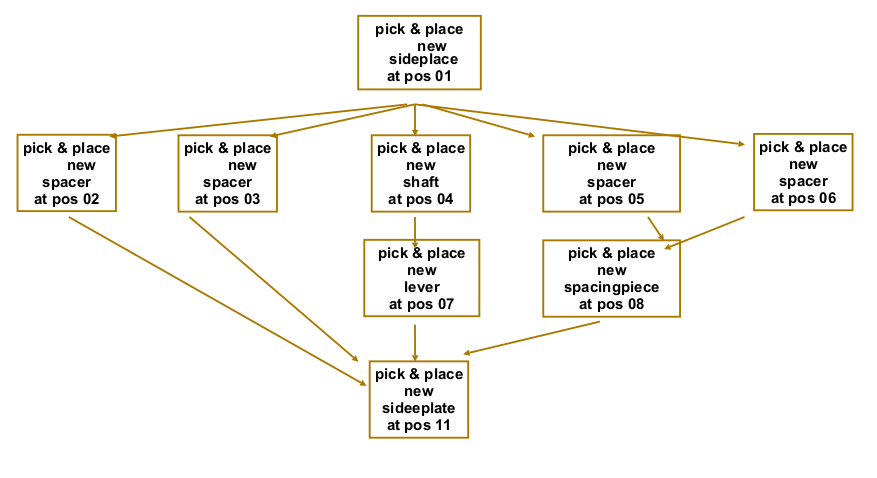
\includegraphics[width=\textwidth]{figures/ch02_vg-bsp.png}
		\caption{Beispiel: Vorranggraph des Cranfield-Benchmarks (simple Montage-Aufgabe)}
		\label{vg}
	\end{subfigure}
	\caption{Vorranggraph}
	\label{vg1}
\end{figure}
\begin{itemize}
\item Darstellung der Handlung in mehreren unabhängigen Teilzweigen
\item Üblicherweise: Serialisierung notwendig!
\begin{itemize}
\item Berechnung optimaler Operatorreihenfolgen
\item Freiheitsgrad zum Ausführungszeitpunkt
\item Serialisierung aufwendig ($\rightarrow$ Planungsverfahren, siehe spätere Vorlesungen)
\end{itemize}
\item Ausführung beinhaltet also:
\begin{itemize}
\item Serialisierung der Handlung nach gegebenen Kriterien
\item Ausführung der sequentiell beschriebenen Handlung
\end{itemize}
\item Mächtigere Handlungsbeschreibung benötigt auch mächtigere Verfahren bei der Ausführung!
\end{itemize}
\textbf{Hierarchisches Aufgabenmodell} (Abbildungen \ref{hier} und \ref{hiermod}):\\
Sowohl Aufgabenspezifikation als auch Aufgabenzerlegung/-teilung sind hierarchisch strukturiert. Die Abstraktion erfolgt nach Raum, Zeit, Objekten und Alternativen.
\begin{figure}[h!]\centering 
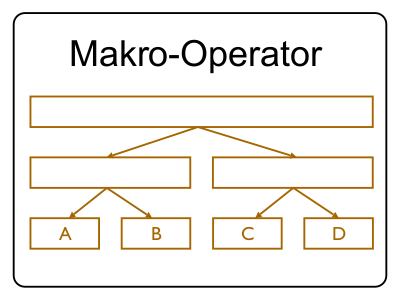
\includegraphics[width=0.3\linewidth]{figures/ch02_hier.png}
\caption{}
\label{hier}
\end{figure}\\
\begin{figure}[h!]
	\centering
	\begin{subfigure}{.45\textwidth}
		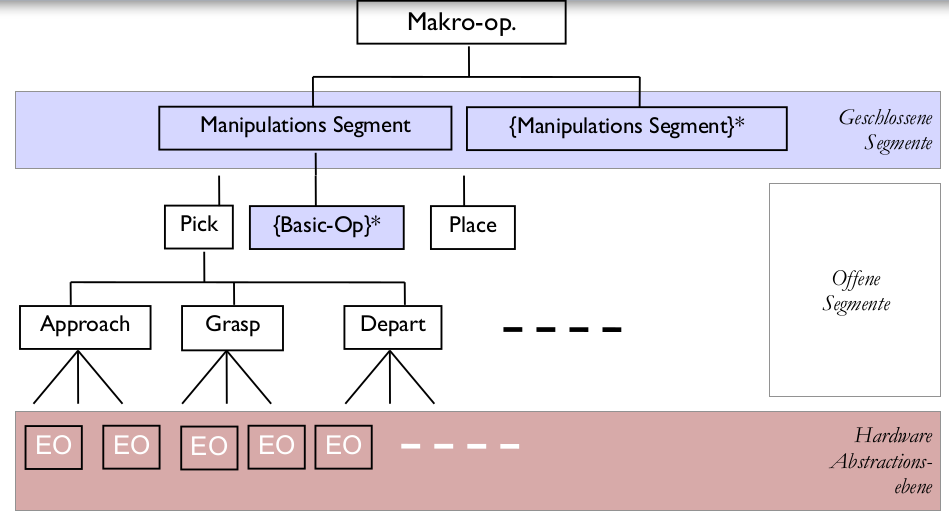
\includegraphics[width=\textwidth]{figures/ch02_hier1.png}
		\caption{Semantische hierarchische Repräsentation}
	\end{subfigure}
	\begin{subfigure}{.45\textwidth}
		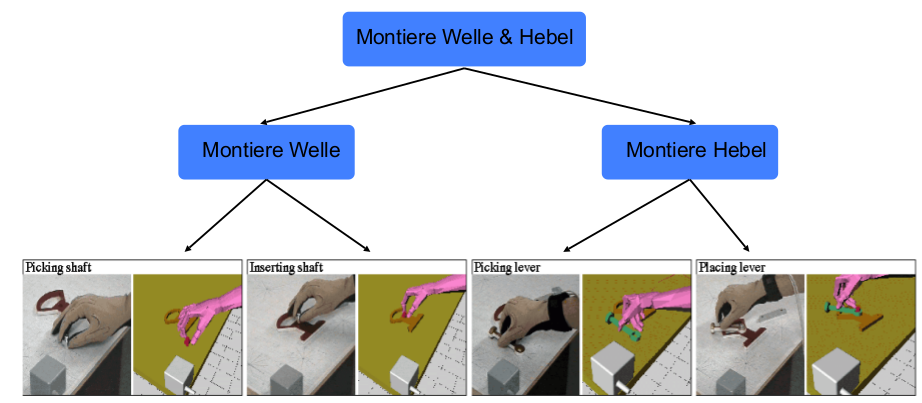
\includegraphics[width=\textwidth]{figures/ch02_hier2.png}
		\caption{Programmbeispiel: Montage von Welle und Hebel des Cranfield Benchmarks}
	\end{subfigure}
	\caption{Hierarchisches Aufgabenmodell}
	\label{hiermod}
\end{figure}
\paragraph*{Abstraktionsebenen im Aufgabenmodell}
Häufige Unterscheidung der in \autoref{abst} dargestellten semantischen Abstraktionsstufen. Diese benutzen symbolische Parameter.
\begin{itemize}
\ita Komplexität der Aufgabe beherrschbar
\ita Formalismen anwendbar
\end{itemize}
\begin{figure}[h!]\centering 
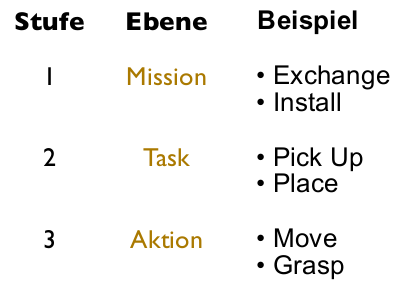
\includegraphics[width=0.3\linewidth]{figures/ch02_abst.png}
\caption{}
\label{abst}
\end{figure}
\textbf{Wahl der Abstraktionsebene}: Wie wird die Abstraktionsebene der Aktion gewählt, damit Aktionen von Roboter A auf Roboter B übertragen werden können?
\begin{itemize}
\item Aktion: Kleinste symbolische Einheit
\item Darunter: Regelungsebene
\item Abhängig von:
\begin{itemize}
\item Komplexität der Aufgabe
\item Grad der Kopplung einzelner Teilhandlungen
\item Hardware: Getrennt geregelte Komponenten werden üblicherweise auch mit getrennten Aktionen modelliert
\item Planungssystem/Beobachtungssystem
\end{itemize}
\item Grundsätzlich: Die Frage ist in der Forschung noch nicht eindeutig geklärt, immer noch ein Streitpunkt!
\end{itemize}
\textbf{Modellierung von Aktionen / Tasks}:\\
Ein \textcolor{red}{Operator} ist definiert durch $OP = (N, O, A, Par, K)$ mit
\begin{itemize}
\item $N$ = Name des Operators (eindeutig)
\item $O$ = Liste der beteiligten Objekte
\item $A$ = Auswahlbedingung
\item $Par$ = Liste der Parameter, z.B. Positionen, Kräfte, Beschleunigungen ...
\item $K$ = Körper des Operators:
\begin{itemize}
\item \textcolor{red}{\textbf{Aktion}/Elementaroperator}:\\ ausführbares Programm\\ $\Rightarrow$ Realisierung einfacher Fähigkeiten
\item \textcolor{red}{\textbf{Task}/Makro-Operator}:\\ besteht aus weiteren Operationen $K = K_1K_2...K_n$ $\Rightarrow$\\ Realisierung einfacher Fähigkeiten
\end{itemize}
\end{itemize}
\textbf{Hierarchische Repräsentation -- Ausführung}:
\begin{itemize}
\item Im Aufgabenmodell ist die Serialisierung implizit gegeben
\begin{itemize}
\item Minimaler Aufwand zur Ausführung
\item Aber: Bei Parallelitäten von Teilhandlungen: Konflikte möglich!
\end{itemize}
\item Ausführung beinhaltet also:
\begin{itemize}
\item Überprüfung auf Konflikte
\item Gegebenenfalls Serialisierung/Lösen der Konflikte
\item Ausführung der resultierenden Operatorsequenz
\end{itemize}
\item Vorteil: Zusammengesetzte (Teil-)Programme können wiederverwendet werden
\item Repräsentation gut \glqq lesbar\grqq{} (verständlich, erklärbar)
\end{itemize}
\textbf{Anwendung hierarchischer Handlungsbeschreibung in der Realität  \\-- Flexible Programme}:\\
Symbolische Abstraktionsebene zur Roboterprogrammierung
\begin{itemize}
\item Hierarchische Handlungsbeschreibung
\item Erklärbar, verständlich, intuitiv
\item Wiederverwendbarkeit
\item Parametrierbar
\item Unterstützt: Bedingungen, Verzweigungen, Ressourcenverwaltung, Parallelität
\item Aufbau flexibler Programme:
\begin{itemize}
\item Repräsentation des Handlungswissens als Baumstruktur
\item Parametrierbare Aktionsbeschreibung
\item Blätter entsprechen Roboteraktionen
\item Abarbeitung entsprechend einer Tiefensuche
\item Instantiierung der Kinder zur Laufzeit (Expansion des Baums)
\item Auswahl des geeignetsten Kandidaten beim expandieren
\item Parallele Ausführung mehrerer Kinder möglich
\end{itemize}
\end{itemize}
\paragraph*{Validierung der Modelle: Simulation oder Graphische Animation}
\begin{enumerate}
\item \textbf{Simulation der Komponenten}: Validierung anhand gegebener Einschränkungen (Kollisionen, Erreichbarkeit, Optimalitätskriterien: Weg, Zeit, Energie, ...)
\begin{itemize}
\ita Für die Simulation von Effekten durch Manipulators wird die Physiksimulation verwendet: Masse, Reibung, Kräfte, Gelenke
\end{itemize}
\item \textbf{Graphische Animation}: Der Anwender überprüft visuell die erstellten Modelle
\begin{itemize}
\ita Wenn die Robotersimulationen ergeben, dass die Zielstellung angefahren werden kann, wird die Bewegung in einer Animation graphisch dargestellt.
\end{itemize}
\end{enumerate}

\paragraph*{Aufgabenmodell -- Zusammenfassung und Diskussion}:\newline
\textbf{Zusammenfassung}:
\begin{itemize}
\item Aufgabenmodell basiert auf elementaren Operationen
\item Oft dreischichtiger Ansatz: Aktion, Task, Mission
\item Verknüpfung der elementaren Operationen zu komplexen Aufgaben:
\begin{itemize}
\item Sequentiell
\item Vorranggraph
\item  Hierarchisch
\item (Kontrollstrukturen)
\end{itemize}
\item Problem: Validierung der Programme
\begin{itemize}
\item Simulation
\item Animation und Validierung durch den Menschen
\end{itemize}
\end{itemize}

\textbf{Diskussion}:
\begin{itemize}
\item Mobile Plattform ohne Sensorik (z.B. Roomba)
\begin{itemize}
\item Aufgabenmodell?
\item Umweltmodell?
\end{itemize}
\item Mobile Plattform mit Differentialantrieb und Sensorik zur Lokalisation (z.B. Transportaufgaben)
\begin{itemize}
\item Aufgabenmodell?
\item Umweltmodell?
\end{itemize}
\item Serviceroboter mit mobiler Plattform, Manipulator, Mehrfingergreifer, komplexe Sensorik\begin{itemize}
\item Aufgabenmodell?
\item Umweltmodell?
\end{itemize}
\item Wo kommt jeweils das Aufgabenwissen dieser Systeme her?
\end{itemize}

\section{Interaktive Programmierung: Programmierung durch Vormachen von Manipulationsaufgaben} %(3.-5. VL)
\subsection{Grundlagen}
Neue Anforderungen an Robotersysteme:
\begin{itemize}
\item In der Produktion: Klein- \& Kleinstserienfertigung, Unikatfertigung (z.B. Prototyp)\\
$\rightarrow$ Produkte mit: vielen Ausstattungsvarianten und hoher Rekonfigurierbarkeit\\
$\rightarrow$ Flexible Fertigung
\item Im Servicebereich: \\
$\rightarrow$ Handel:  Kommissionierung und Palettierung von Waren, Bestücken von Regalen\\
$\rightarrow$ Pflege: Unterstützung von Rehabilitationsmaßnahmen durch Roboter, Rollstuhl mit Manipulationshilfe\\
$\rightarrow$ Handwerk: Handhabungen in Schreinereien und Schlossereien
\item In der humanoiden Servicerobotik: Manipulation beliebiger Objekte, selbstständiges Lösen komplexer Aufgaben, Einsatz im menschlichen Umfeld\\
$\rightarrow$ komplexe Umgebung und sehr viele Freiheitsgrade\\
$\rightarrow$ Wie Handlungswissen erzeugen?
\end{itemize}

\subsubsection*{Grundidee der interaktiven Programmierung} %5.1.1.
\begin{itemize}
\item[1.]Mensch ist Domänenexperte (Manipulation)
\item[2.]Explizite Demonstrationen der Manipulationsaufgabe
\item[3.]Sensorielle Erfassung der Demonstrationen
\item[4.]Erzeugung der internen Repräsentation des Roboterprogramms
\item[5.]Abbildung auf das Robotersystem
\item[6.]Ausführung
\end{itemize}

\subsubsection*{Anforderungen an interaktive Programmierung}
\begin{itemize}
\item[1.]Intuitive Interaktionsformen: einfache Bedienung des Systems
\item[2.]Transparenz der Prozesse im Programmiersystem: Umsetzung von Handlungen des Benutzers soll nachvollziehbar sein
\item[3.]Abgleich von Systemhypothesen mit der Benutzerintention: z.B. zur Korrektur falscher Systemhypothesen
\item[4.]Flexibilisierung und Optimierung von Programmen: erlernte Programme sollen in vielen Situationen anwendbar sein
\item[5.]Wiederverwendung von Teillösungen: Funktionsbausteine sollen in anderen Pogrammen wiederverwendbar sein
\end{itemize}

\subsubsection*{Randbedingungen}
Notwendig zur Erzeugung von leistungsfähigen, automatischen aber auch sicheren und komfortablen Roboterprogrammen
\begin{itemize}
\item[1.]Weitgehend automatisierte Programmgenerierung
\item[2.]Beschränkung der Benutzerinteraktion auf das Nötigste
\item[3.]Maximierung des Informationsgewinns und der Eindeutigkeit der Ergebnisse der Benutzerinteraktion für das System
\item[4.]Möglichst benutzerfreundliche Mensch-Maschine Interaktion: verständlich, transparent und flexibel, möglichst ähnlich zur zwischenmenschlichen Kommunikation
\end{itemize}

\subsection{PdV - Generelles Framework}
\begin{figure}[ht]\centering 
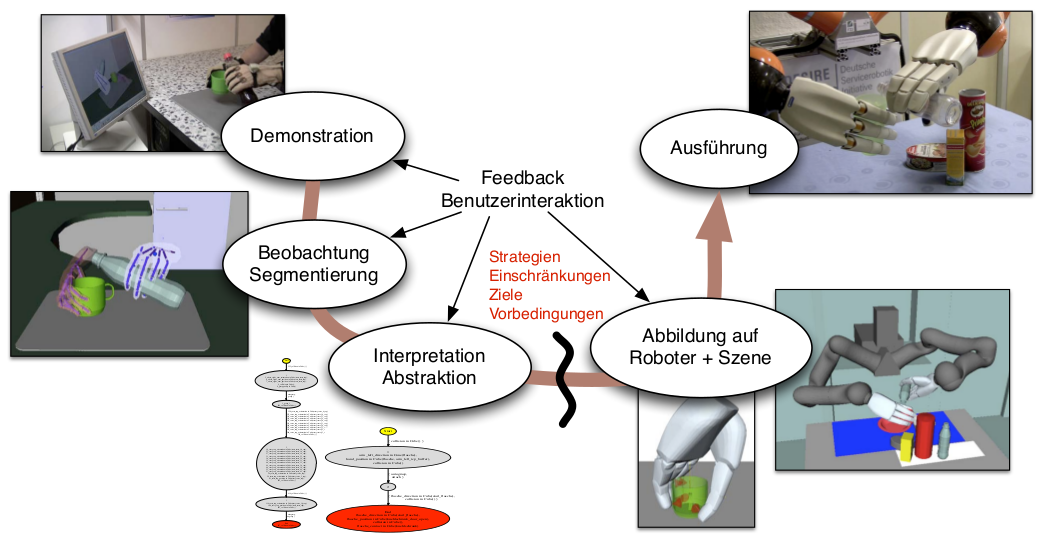
\includegraphics[width=0.6\linewidth]{figures/ch03_zyklus.png}
\caption{PdV-Zyklus}
\label{fig:ch03_zykl}
\end{figure}
Abbildung  \ref{fig:ch03_zykl} zeigt die Phasen von PdV.
\subsubsection*{Beobachtung}
Beobachtung der Benutzerinteraktion mittels externer und interner Sensorik (z.B. Kamerasysteme, Datenhandschuhe, Positionstracker).
\begin{itemize}
\ita mit den gewonnenen Sensordaten lassen sich dann Objekte klassifizieren, Trajektorien aufzeichnen und weitere Vorverarbeitungsschritte wie
Grifferkennung durchführen
\end{itemize}

\subsubsection*{Segmentierung}
Segmentierung in relevante Operationen oder Umweltzustände. 
\begin{itemize}
\item man benötigt hierfür die Trajektorien aus der Demonstration, eine Datenbasis mit den Sensordaten, einen Satz Aktionstypen (Griffe, Lageänderungen von Objekten), einen Satz
von Elementaroperationen und das Umweltmodell
\item durch eine geeignete Heuristik lässt sich damit die Segmentierung durchführen
\item eine zusätzlich Interaktion mit dem Benutzer (über verschiedene Kommunikationskanäle wie grafische Benutzerschnittstellen oder Sprache) hilfreich; 
Rückfragen helfen bei der Identifikation der in der Lösung involvierten Objekte und sparen damit unnötige Berechnungen aller Relationen zwischen allen Objekten
ein
\item Rauschfilterung
\end{itemize}
\subsubsection*{Interpretation/Abstraktion}
Abstraktion von der Demonstration um die Lösung der Aufgabe so allgemein wie möglich darzustellen.
\begin{itemize}
\ita Instanzen müssen falls möglich in Variablen umgewandelt werden; dabei muss sichergestellt werden, dass in der Ausführungsphase nur solche Variablen instantiiert
werden, die räumliche Vorbedingungen erfüllen. Es wird also für jeden \Gu generalisierten\Go Operator ein Satz von Vorbedingungen in Form von wichtigen Relationen
gespeichert. Generiert werden diese Vorbedingungen mit Hilfe von Hintergrundwissen und wiederum durch Rückfragen an den Benutzer. Man benötigt also eine deduktive
Komponente, die die generalisierten Operatoren in Makro-Operatoren gruppiert. Da Makro-Operatoren weitere Makro-Operatoren als Kinder beinhalten können, lässt
sich die gesamte Benutzervorführung auf verschiedenen Abstraktionsebenen darstellen. Durch die Generalisierung lässt sich die Lösung später auf ähnliche Problemklassen anwendbare Lösungsbeschreibungen abbilden. In dieser Phase lassen sich auch vom Demonstrator durchgeführte spontane und nicht zielorientierte Bewegungen ausfiltern.
\end{itemize}
\subsubsection*{Transfer/Abbildung auf Roboter \& Szene}
Transfer der internen Wissensrepräsentation auf das Zielsystem. Aus den zuvor gewonnenen semantischen Informationen lässt sich jetzt ein ausführbares Roboterprogramm generieren. Dafür müssen die Operationen auf die Operationen des Zielsystems abgebildet werden. Die Ausgabe dieser Phase ist eine Sequenz von Elementarbewegungen, die nur für das Zielsystem und das jeweilige Umweltmodell gültig sind. Diese kann direkt in das Simulationsmodul weitergeleitet werden.
\subsubsection*{Simulation}
Simulation des physikalischen Vorgangs zur Validierung der getroffenen Entscheidungen. In der Simulation wird die gelernte Aufgabe von einem virtuellen Modell des Roboters in einer virtuellen Umwelt an virtuellen Objekten ausgeführt. Anhand einer visuellen Ausgabe lässt sich vom Benutzer die korrekte Ausführung der Aufgabe überprüfen. 
\subsubsection*{Ausführung}
Ausführung auf dem Zielsystem. Die zuvor validierte Sequenz elementarer Roboterbewegungen wird an den Roboter-Controller weitergereicht. Wenn bei der Modellierung in der Simulationsphase keine Fehler gemacht wurden, ist es sehr wahrscheinlich, dass die Ausführung nicht fehlschlagen wird-

\subsection{Klassifikation von PdV-Verfahren}
\begin{figure}[ht]\centering 
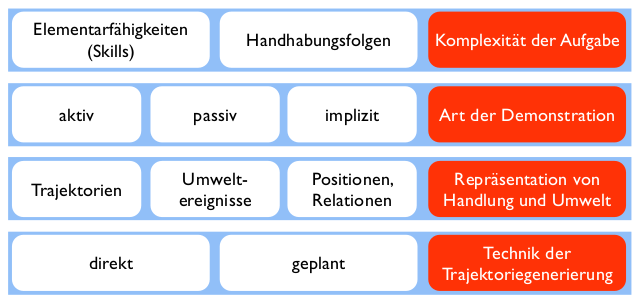
\includegraphics[width=0.6\linewidth]{figures/ch03_kriterien.png}
\caption{Klassifikationskriterien}
\label{fig:ch03_krit}
\end{figure}
Abbildung  \ref{fig:ch03_krit} zeigt die Klassifikationskriterien auf einen Blick.
\subsubsection*{Komplexität der Aufgabe}
Siehe Tabelle \ref{tab:aufgkomp}
\begin{table}[hbt]
\centering
\begin{tabular}{|p{8cm}|p{8cm}|}
\hline
Elementarfähigkeiten & Komplexe Aufgaben\\
\hline
Reflexe, Basisskills, einfache Bewegungen 
\vspace{-4mm}
\begin{itemize}
\setlength\itemsep{0em}
\item Lernen direkter Sensor-/Aktorzusammenhänge
\item Beispiele: Verwendung neuronaler Netze auf adaptive Regelkreise, Zustandsautomaten \footnote{Asada91, Koeppe95, Kaiser96, Ishikawa99, Bentivegna00, Calinon08, Pastor09}
\item[$\rightarrow$] Probleme: Explizite Beispiele, stark konfigurationsabhängig,
viele Trainingsbeispiele notwendig
\end{itemize}
 &
Task, Montageaufgaben
 \vspace{-4mm}
\begin{itemize}
\setlength\itemsep{0em}
\item Interpretation von Handlungsfolgen\footnote{Segre89, Inaba90, Kang94, Sagerer98, Aleotti06, Pardowitz07
Veeraraghavan08}
\ita Probleme: Breites Hintergrund-, Planungs- und Modellwissen,
Klärungsdialoge mit dem Benutzern
\end{itemize}\\
\hline
\end{tabular}
\caption{Kriterium 1 - Komplexität der Aufgabe}
\label{tab:aufgkomp}
\end{table}
\subsubsection*{Art der Demonstration}
Siehe Tabelle \ref{tab:demo}
\begin{table}[hbt]
\centering
\begin{tabular}{|p{5cm}|p{5cm}|p{5cm}|}
\hline
aktiv & passiv & implizit\\
\hline
Aktive Beispiele
\vspace{-4mm}
\begin{itemize}
\setlength\itemsep{0em}
\item Benutzer führt explizit vor
\item Beobachtung durch Sensorsystem (Datenhandschuh, Kameras)\footnote{Friedrich98, Ikeuchi99, Inoue/Kuniyoshi94, Zöllner06}
\ita Probleme: Aufwendige Sensorsysteme, Identifikation relevanter Aktionen und Ziele bzw. Zustände schwierig
\end{itemize}
 &
Passive Beispiele
 \vspace{-4mm}
\begin{itemize}
\setlength\itemsep{0em}
\item Roboter wird duch externen \Gu Master\Go
gesteuert, Signalaufzeichnung, Korrelation
zwischen Sensor- und Aktordaten\footnote{Kaiser96, Koeppe98, Billard07}
\ita Probleme: Gelerntes Wissen ist auf
konkretes Zielsystem festgelegt
\end{itemize} 
&
Implizite Beispiele
 \vspace{-4mm}
\begin{itemize}
\setlength\itemsep{0em}
\item Zielspezifikation durch Vorgabe graphischer Ikone\footnote{Takahashi/Ogata97,Sagerer98, Riepp97}
\ita Probleme: Dialog umfangreich, Anpassung an Zielsystem
\end{itemize}\\
\hline
\end{tabular}
\caption{Kriterium 2 - Art der Demonstration}
\label{tab:demo}
\end{table}

\subsubsection*{Repräsentation von Handlung und Umwelt}
Siehe Tabelle \ref{tab:rep}
\begin{table}[hbt]
\centering
\begin{tabular}{|p{5cm}|p{5cm}|p{5cm}|}
\hline
Trajektorien & Umweltereignisse & Positionen, Relationen\\
\hline
\vspace{-4mm}
\begin{itemize}
\setlength\itemsep{0em}
\ita Problem: keine wesentliche Generalisierung (1:1 Abbildung)
\end{itemize}
 &
Wirkungen und Reaktionen auf die Umgebung
 \vspace{-4mm}
\begin{itemize}
\setlength\itemsep{0em}
\ita Probleme: Identifikation von Kausalitäten und
Zustandsfolgen durch kognitive Operatoren
\end{itemize} 
&
Objektlagen, Relationen und Operatoren
 \vspace{-4mm}
\begin{itemize}
\setlength\itemsep{0em}
\ita Probleme: Beschränkung auf vorgegebenen
Operatorumfang
\end{itemize}\\
\hline
\end{tabular}
\caption{Kriterium 3 - Repräsentation von Handlung und Umwelt}
\label{tab:rep}
\end{table}
\subsubsection*{Technik der Trajektoriengenerierung}
Siehe Tabelle \ref{tab:trajtech}
\begin{table}[hbt]
\centering
\begin{tabular}{|p{8cm}|p{8cm}|}
\hline
direkt & geplant\\
\hline
Planung von Roboterbewegungen / Aktionen
\vspace{-4mm}
\begin{itemize}
\setlength\itemsep{0em}
\item Planung erforderlich zur Berücksichtigung der Unterschiede in
Demonstrations- und Ausführungsumgebung
\item Vollständige Nutzung der Leistungsfähigkeit des Robotersystems
\ita Probleme: Umwelt- und Planungswissen erforderlich,
intelligentes Planungssystem
\end{itemize}
 &
Direkte Abbildung
 \vspace{-4mm}
\begin{itemize}
\setlength\itemsep{0em}
\item Explizites oder gelerntes Transformationsmodell\footnote{Kang97, Kaneko97}
\ita Probleme: Zielsystem und Zielumgebung müssen korrespondieren
\end{itemize}\\
\hline
\end{tabular}
\caption{Kriterium 4 - Technik der Trajektoriegenerierung}
\label{tab:trajtech}
\end{table}

\subsection{Prozesskomponenten der interaktiven Programmierung}
\begin{figure}[ht]\centering 
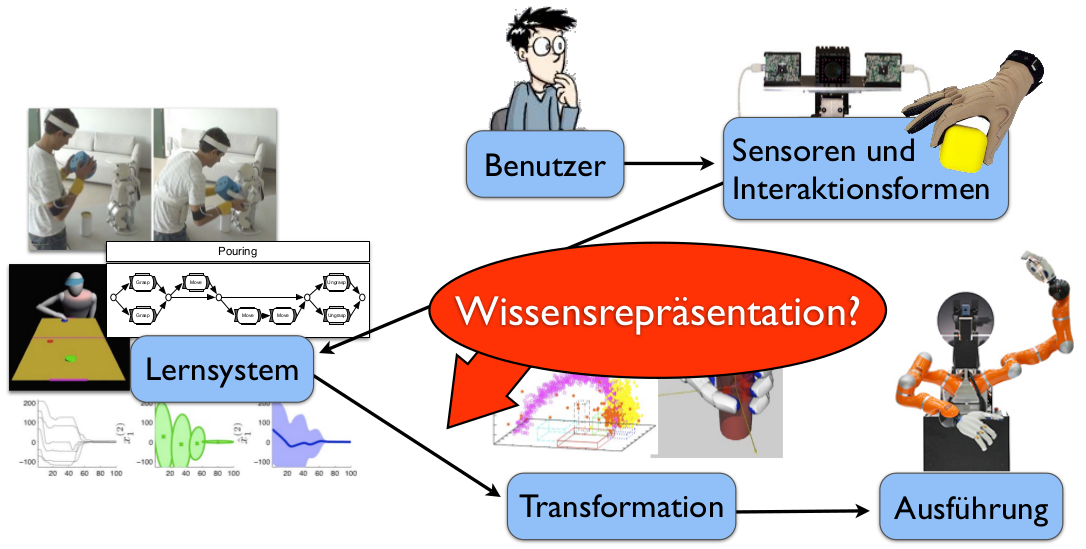
\includegraphics[width=0.6\linewidth]{figures/ch03_komponenten.png}
\caption{Interaktive Programmierung: Komponenten}
\label{fig:ch03_kom}
\end{figure}
Abbildung \ref{fig:ch03_kom} skizziert die an PdV beteiligten Komponenten:
\subsubsection*{Benutzer und Mensch-Maschine-Interaktionsformen}
Der Mensch, welcher die interaktive Programmierung vornimmt, kann multimodal mit dem Programmiersystem interagieren:
\begin{itemize}
\item \textbf{Physische Demonstration:}
Hierbei vollzieht der Benutzer die Manipulationsaufgabe mit realen Objekten und wird dabei
vom Programmiersystem durch Sensoren erfasst und seine Handlungen aufgezeichnet. 
Dies ist die natürlichste Art der Demonstration: Objekte können direkt mit den Händen 
oder mittels spezieller Vorführgeräte (z.B. Laserstift, 6D-Kugel) manipuliert werden. 
In jedem Fall ein großes Maß an Konzentration auf Seiten des Benutzers gefordert\\
Nachteile: 
\begin{itemize}
\item[-]Er muss sich weiterhin über die Beschränkung und Konfiguration der ihn beobachtenden Sensoren bewusst sein
(z.B. Verdeckung bei Beobachtung durch eine Kamera). Wegen der Abtastfrequenz der Sensoren
ist auch die Geschwindigkeit, mit der die Demonstration vorgeführt wird, zu beachten.
Oft ist es auch sinnvoll, die Manipulationsaufgabe in Teillösungen zu untergliedern, um
gegebenenfalls Fehler leichter zu beheben.
\item[-] Aufgrund der beschränkten sensorischen,
motorischen und intellektuellen Fähigkeiten des Menschen kann keine absolute 
Positioniergenauigkeit erwartet werden und auch die Wiederholgenauigkeit ist begrenzt.
\item[-] Auch produzieren menschliche Benutzer schon bei einfachen Manipulationsaufgaben häufig ineffiziente
oder überflüssige Handlungen. Ebenfalls tragen der Umfang und die Komplexität der Demonstration
der zu programmierenden Aufgabe dazu bei.
\end{itemize}
\item \textbf{Graphische Demonstration:} 
Der Benutzer kann hierbei die Manipulationsaufgabe lösen,
indem er 3D Objekte in einer simulierten Umgebung bewegt. Einige Probleme der physischen
Demonstration mit Sensoren (eingeschränkte Beobachtbarkeit, limitierte Genauigkeit, zeit-
licher Aufwand) sind bei dieser Art der interaktiven Programmierung nicht vorhanden. Es
wird versucht, die Vorteile der intuitiven physischen Demonstration zu übernehmen und
die angesprochenen Nachteile zu umgehen. Leider entstehen bei dieser Art von Demonstration
andere Probleme. Auf einem Monitor ist die Wiedergabe einer 3D Szene mit ihren zu manipulierenden
Objekten nur schwer zu erfassen. Sollen nur Translationen und Rotationen in einer Ebene ausgeführt
werden (z.B Bestückung einer Platine) reicht ein Monitor aus. Besser eigenen sich für die Darstellung
von 3D Umgebungen Datenhelme und Shutter Brillen sowie 3D Höhlen. Mit den
bisher beschriebenen Hilfsmitteln zur interaktiven Programmierung ist keine Möglichkeit
der Kraftrückkopplung gegeben. Haptischen Ein- und
Ausgabegeräte (Datenhandschuh mit Exoskelett und Phantom Manipulator) ermöglichen die Reaktionskräfte
an den Benutzer weiterzugeben. Er kann besser auf die simulierte Welt
einwirken, da er ein Feedback bekommt. Wegen der Echtzeitmodellaktualisierung ist aber
ein hoher Rechenaufwand nötig.\\
Diese ist für den menschlichen Benutzer mit den gleichen
Problemen verbunden wie die physische. Hinzukommen Probleme der Navigation und Koordination
in der simulierten Umgebung. Aufgrund der fehlenden Realität der virtuellen
Welt kann es sogar zu Simulationsübelkeit kommen. Dies geschieht durch den Widerspruch
der Signale, welche vom Gleichgewichts-, Orientierungs-, Seh- und Gehörsinn aufgenom-
men werden.
\item \textbf{Symbolische/Ikonische Demonstration:}
Es wird eine Aktionssequenz erzeugt, durch graphisches Aneinanderreihen vorhandener Teillösungen. 
Für diese Art der Demonstration reicht eine menügesteuerte, konventionelle graphische Schnittstelle.
Es müssen nur entsprechende Operatoren vorhanden sein, welche alle Informationen zur Manipulation
einzelner Objekte beinhalten. Die Ressourcenanforderungen an das System sind dementsprechend gering.
Bei ihr setzt der menschliche Benutzer aus
vorhandenen Teillösungen eine Lösung für die Manipulationsaufgabe zusammen. Das Problem
ist hierbei die Bestimmung der zu manipulierenden Objekte und die Parametrisierung
der Bewegungsfolge.
Die Kommentierung von Systemhypothesen, die Vermittlung der Sensorik von Aktionen
und der eigenen Intention ist für den Benutzer bei entsprechenden Benutzerschnittstellen
(symbolische, graphische Darstellung) leichter.
\item \textbf{Kommentierung:} Sie ist eine ergänzende Interaktionsform zur physischen oder 
graphischen Programmierung. Der Benutzer nimmt hierbei keine aktive Rolle ein, sondern reagiert
auf Systemhypothesen. Nach einer Demonstration erhält man die Möglichkeit, Systemhypothesen zu
präsentieren und durch Auswahl, Editierungen und Ablehnung mit der
Benutzerintension abzugleichen.
In vielen Anwendungen (Textverarbeitung, Graphikanwendungen, Programmierung) sind
textuelle oder menüubasierte Schnittstellen ausreichend. In der Robotik kann es durch den
rämlichen Bezug der Systeme zusätzlich nötig sein, über zweidimensionale graphische
Interaktionsmuster hinaus eine dreidimensionale Schnittstelle zu bieten. Nur mit 
Kommentierung ist eine Überwachung und gegebenenfalls eine Korrektur der systeminternen
Programmgenerierung möglich.
\end{itemize}
\subsubsection*{Sensoren}
\begin{itemize}
\item \textbf{Bildgebende Sensoren}: meist Kameras; ermöglichen zusätzlich zur Aufnahme und Analyse der Demonstration eine Modellierung der Umwelt, kritisch hierbei ist der hohe Rechenaufwand und Schwierigkeiten für den Benutzer (muss im optimalen Bildbereich agieren und Verdeckungen zwischen Hand und Zielobjekt vermeiden)
\item \textbf{Magnetfeldbasierte Positionssensoren}: direkte Bestimmung von Position und Orientierung der Benutzerhand; Erkennung nicht durch Verdeckungen und Lichtverhältnisse behindert; problematisch ist die quadratische Abnahme der magnetischen Feldstärke und Störungen durch metallische Gegenstände
\item \textbf{Datenhandschuhe \& -anzüge}: Dehnmessstreifen und Lichtleiter; niedrige Genauigkeit 
\item \textbf{Exoskelette}: höhere Genauigkeit durch mechanische Struktur aber hohe Kosten, Gewicht, Einschränkung des Benutzers bei der Demonstration  
\item \textbf{Interne Robotersensoren}: zuverlässige Werte (wenn für Demonstration und Ausführung derselbe Roboter verwendet wird ist bei gleicher Umweltsituation der erfolg garantiert) aber hoher Geräteaufwand und geringer Komfort für Benutzer, daher eher bei Teach-In und Telerobotik verwendet
\item[$\rightarrow$] Sensordatenfusion sinnvoll, aber ihrerseit mit Herausforderungen behaftet
\end{itemize}
\subsubsection*{Weltmodell sowie Planungs- und Entscheidungsmechanismen/ Programmiersystem}
\begin{figure}[ht]\centering 
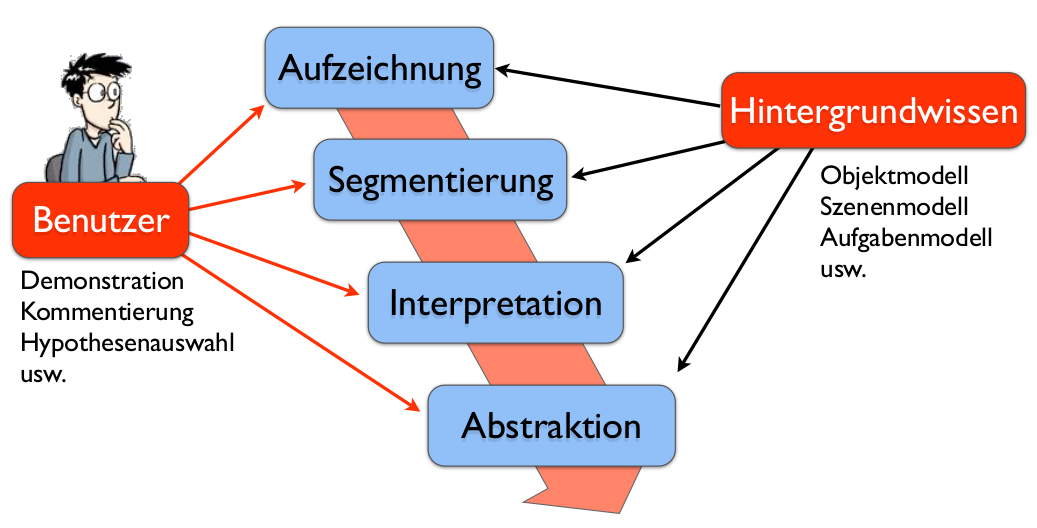
\includegraphics[width=0.6\linewidth]{figures/ch03_verarbeitungsschritte.png}
\caption{Lernsystem: Verarbeitungsschritte}
\label{fig:ch03_verarb}
\end{figure}

Abbildung \ref{fig:ch03_verarb} zeigt die Berarbeitungsschritte eines interaktiven Programmiersystems
%F18 ??
\subsubsection*{Ausführende Manipulatoren}
Ein Manipulator ist ein Roboter, der sich aus einer Steuerung und mechanischen Komponenten (Manipulatorarm) zusammen setzt. Er ist in der Lage, die Position und Orientierung
eines Objektes bezüglich eines Bezugskoordinatensystems zu ändern.
Es sind zwei Arten der Wissensrepräsentation zu unterscheiden, wie in Tabelle \ref{tab:Wissrep} dargestellt.

\begin{table}[hbt]
\centering
\begin{tabular}{|p{8cm}|p{8cm}|}
\hline
Manipulatorabhängige Repräsentation: \newline \textcolor{red}{subsymbolisch} & Manipulatorunabhängige Repräsentation: \newline \textcolor{red}{symbolisch}\\
\hline
Angabe von
\vspace{-4mm}
\begin{itemize}
\setlength\itemsep{0em}
\item Aktionssequenz oder
\item Gelenkwinkel-, Kraft und Momenttrajektorien
\end{itemize}
Nachteile: 
\begin{itemize}
\setlength\itemsep{0em}
\item[-] bei Serviceanwendungen nicht flexibel genug, da invariante Trajektorien keine Veränderung der Lage zu den manipulierten
Objekten in der Umwelt erlauben
\item[-] Variationen in Material, Form und Gewicht beim Manipulationsobjekt können nicht berücksichtigt werden; statische Trajektorien verlieren bei einer Veränderung dieser Werte zur
Programmausführung ihre Gültigkeit
\item[-] unterschiedliche Manipulatoren weisen aufgrund der Kinematik der Manipulatorarme und Endeffektoren verschiedene Konfigurationsräume auf und besitzenverschiedene Sensorausstattung
\item[-] bei expliziter Trajektorienerfassung benötigt man viel Speicher
\item[$\rightarrow$] durch die schwach strukturierte Umwelt und die Forderung von Wiederverwendbarkeit im Dienstleistungsbereich ist die manipulatorabhängige Repräsentation hier nicht sinnvoll
\end{itemize}
 &
 Angabe von Sequenzen von Elementaroperatoren
 \vspace{-4mm}
\begin{itemize}
\setlength\itemsep{0em}
\item Elementaroperatoren sind Regelungen mit Start-, End- und Fehlerkriterien
\item Implementierung der Elementaroperatoren ist manipulatorunabhängig
\item Effekte in der Umwelt sind manipulatorunabhängig, Situation wird nur über lokale Sensorwerte erstellte Umweltinformation beschrieben
\end{itemize}
Bewertung:
\begin{itemize}
\setlength\itemsep{0em}
\item[+] flexible Repräsentation und benutzerfreundliche symbolische Darstellung
\item[+] größere Flexibilität gegenüber Umweltveränderungen und unterschiedlichen Manipulatortypen
\item[+] Elementarfunktionen haben einen hohen Wiederverwendbarkeitswert, so braucht ein Programm nur die Sequenz der Elementarfähigkeiten
enthalten und ihre einzelnen Parameter bestimmen und repräsentieren;  oft weichen in einer
dynamischen Welt die Parameter der Elementarfähigkeiten von denen der Benutzerdemonstation ab, daher werden für variable Parameter Berechnungsfunktionen und
Auswahlbedingungen statt konkreter Werte benutzt
\item[-] Elementarfähigkeiten müssen für jeden Manipulator a-priori erzeugt werden 
\end{itemize}\\
\hline
\end{tabular}
\caption{Arten der Wissenrepräsentation}
\label{tab:Wissrep}
\end{table}

%Tabelle 5.1 Skript!!
\subsection{Wissensrepräsentation: Beispielsysteme}
\subsubsection*{Probabilistisch (Calinon \& Billard)}\footnote{[Calinon07]: What is the teacher’s role in robot programming by demonstration?\\
On learning, representing and generalizing a task in a humanoid robot}
Ziel: Lernen von Skills, z.B. Schachfigur bewegen
\begin{itemize}
\item Aktive, physische Demonstration am Roboter $\rightarrow$ kein Korrespondenzproblem
\item Repräsentation durch Gaussian Mixture Models (GMM) $\rightarrow$ subsymbolisch
\item Direkte Ausführung
\end{itemize}
Hierbei werden folgende Lerndaten benötigt:
\begin{itemize}
\item $(\theta, x, y, h)$: $n$ Demonstrationen mit je $T$ Trajektoriepunkten
\item $\theta$: Gelenkwinkel des Roboters + Zeitstempel
\item $x$: Kartesische Position der Hände + Zeitstempel
\item $y$: Distanzvektor der Hände zur Startposition des Objekts + Zeitstempel
\item $h$: Binärer Zustand des Greifers (offen, geschlossen) + Zeitstempel
\end{itemize}
Das Lernverfahren besteht dann aus folgenden Schritten: 
\begin{itemize}
\item Dimensionsreduktion und zeitliche Angleichung: $(\theta, x, y, h) \rightarrow (\theta^\prime, x^\prime, y^\prime, h^\prime)$
\item Lernen eines GMMs (vgl. Abbildung \ref{fig:ch03_gmm}) für alle Komponenten, z.B. $x^\prime$ (4-dimensional) mit Dichte $p(x^\prime)$:
\begin{align*}
p(x^\prime) = \sum\limits_{i=1}^k p(i)p(x^\prime|i) = \sum\limits_{i=1}^k \pi_i \mathcal{N}(x^\prime; \mu_i, \Sigma_i)
\end{align*} mit $k$ = Anzahl der Normalverteilungen, $\pi$ = Gewichtung, $\mathcal{N}$ = Normalverteilung
\item Bestimmung von $k$: Bayes‘sches Informationskriterium und EM-Algorithmus
\begin{figure}[ht]\centering 
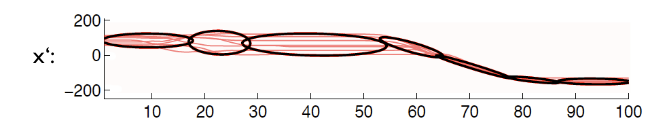
\includegraphics[width=0.6\linewidth]{figures/ch03_gmm.png}
\caption{Gaussian Mixture Model}
\label{fig:ch03_gmm}
\end{figure}
\end{itemize}
Die Repräsentation gestaltet sich folgendermaßen:
\begin{itemize}
\item Probabilistische Darstellung der Trajektorien $x^\prime: t \mapsto \mathcal{N}(\mu_{x^\prime}(t), \Sigma_x(t))$
\item Berechnung durch Gaussian Mixture Regression (vgl. Abbildung \ref{fig:ch03_gmr}): Gewichtung der bedingten Wahrscheinlichkeiten $p(x^\prime, i|t)$
\begin{align*}
\mu_{x^\prime}(t) = \sum\limits_{i=1}^k \beta_i(t)\mu_{i, x^\prime|t} \text{ und } \Sigma_{x^\prime}(t) = \sum\limits_{i=1}^k \beta_i(t)^2\Sigma_{i, x^\prime|t}\\
\text{ mit } p(x^\prime,i|t) = \mathcal{N}(\mu_{i, x^\prime|t}, \Sigma_{i, x^\prime|t}) \text{ und } \beta_i(t) = \frac{p(t|i)}{\Sigma{j=1}^k p(t|j)}
\end{align*}
\begin{figure}[ht]\centering 
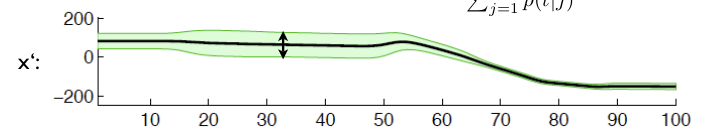
\includegraphics[width=0.6\linewidth]{figures/ch03_gmr.png}
\caption{Gaussian Mixture Regression}
\label{fig:ch03_gmr}
\end{figure}
\end{itemize}
Die Ausführung besteht dann aus folgenden Schritten:
\begin{itemize}
\item Definition eines quadratischen Ähnlichkeitsmaßes: \Gu metric of imitation\Go
\item Gewichtung der Abweichung von den Mittelwerten in $t$, z.B. $\mu_{x^\prime}(t)$
\item Wahl der Gewichtsmatrix: $(\Sigma_{x^\prime}(t))^{-1}$
\item Bestimmung des Nachfolgerzustands $\theta(t+1)$ bzw. der Transition $\theta(t) \rightarrow \theta(t+1)$, die
das Ähnlichkeitsmaß minimiert
\item Jacobi-Matrix zur Kombination von kartesischen und Gelenkwinkeleinschränkungen
\end{itemize}
Eine Bewertung des Verfahrens ist in Tabelle \ref{tab:cabi} dargestellt.
\begin{table}[hbt]
\centering
\begin{tabular}{|p{6.5cm}|p{6.5cm}|}
\hline
Vorteile & Nachteile\\
\hline
\vspace{-5mm}
\begin{itemize}
\setlength\itemsep{0em}
\item[+] schnelles Verfahren, ähnlich Playbackprogrammierung
\item[+] automatische Adaptierung an Änderungen der Objektpositionen
\end{itemize}
 &
 \vspace{-5mm}
\begin{itemize}
\setlength\itemsep{0em}
\item[-] relevante Merkmale manuell definiert, hier z.B. nur Distanz zu Startposition
\item[-] geringe Generalisierung, da keine Vorbedingungen, Ziele, Kollisionen
 keine zielgerichtete Erzeugung von Bewegungen
\item[-] keine Validierung
\end{itemize}\\
\hline
\end{tabular}
\caption{Zusammenfassung: Calinon, Billard}
\label{tab:cabi}
\end{table}\\ 
\subsubsection*{Dynamisch (Pastor \& Schaal)\footnote{[Pastor09]: Learning and generalization of motor skills by learning from demonstration}}
Ziel: Lernen von Skills, z.B. Tennisschwung
\begin{itemize}
\item Aktive, physische Demonstration am Roboter $\rightarrow$ kein Korrespondenzproblem
\item Repräsentation durch Dynamic Movement Primitives (Differentialgleichungen)
\item Direkte Ausführung
\end{itemize}
Die Repräsentation ist wie folgt:
\begin{itemize}
\item Implizite Darstellung durch Menge von Differentialgleichungen:
\begin{align*}
\tau \dot{v} &= K(g-x) -Dv + (g-x_0)f\\
\tau \dot{x} &= v\\
\end{align*}
\item $x$ = Position, $v$ = Geschwindigkeit, $K$ = Federkonstante,
$D$ = Dämpfung, $g$ = Ziel, $x_0$ = Start, $\tau$ = zeitliche Skalierung
\item $f$ = nicht-lineare Funktion, die die Demonstrationsmenge approximiert:
\begin{align*}
f(s) = \frac{\sum_{i=1}^n w_i\psi_i(s)s}{\sum_{i=1}^n \psi_i(s)} \text{ mit } \tau \dot{s} = -\alpha s
\end{align*}
\item Vorteil: Gewichte hängen nicht von $\tau, x_0 $ und $g$ ab
\ita Änderungen von Start, Ziel und der zeitlichen Skalierung möglich
\ita Generalisierung eingeschränkt möglich
\end{itemize}
Das Lernen läuft in folgenden Schritten ab:
\begin{itemize}
\item Berechnung von $v(t), \dot{v}(t)$ für jede Demonstration $x(t)$
\item $s(t)$ wird durch Integration berechnet
\item Der Wert $f(s)$ wird berechnet
\item $\psi_i$ sind nicht normalisierte Normalverteilungen (\Gu Gauss‘sche Basisfunktionen\Go)
\item Bestimmung der Parameter $w_i$ durch lineare Regression
\end{itemize}
Die Ausführung erfolgt über die Berechnung von $v(t), \dot{v}(t)$ im aktuellen Zustand und Integration.\\
Eine Bewertung des Verfahrens ist in Tabelle \ref{tab:pascha} dargestellt.
\begin{table}[hbt]
\centering
\begin{tabular}{|p{6.5cm}|p{6.5cm}|}
\hline
Vorteile & Nachteile\\
\hline
\vspace{-5mm}
\begin{itemize}
\setlength\itemsep{0em}
\item[+] schnelles Verfahren
\item[+] automatische Adaptierung an Start und Ziel
\item[+] lokale Hindernisvermeidung möglich
\end{itemize}
 &
 \vspace{-5mm}
\begin{itemize}
\setlength\itemsep{0em}
\item[-] relevante Merkmale manuell definiert
\item[-] geringe Generalisierung
\item[-] keine Validierung
\end{itemize}\\
\hline
\end{tabular}
\caption{Zusammenfassung: Pastor, Schaal}
\label{tab:pascha}
\end{table}\\ 
\subsubsection*{Sub-/Symbolisch (IPoR II)}
IPor (Interaktives Programmieren von Robotern wurde an der Universität Karlsruhe entwickelt. \\
Problembeschreibung:
\begin{itemize}
\item Robotersystem mit sehr vielen Freiheitsgraden (Kuka LBR / SAH/HIT: 40)
\item  Fingerfertige Manipulation fester Körper („rigid bodies“)
\item Roboterarbeitsraum in realen Situationen stark eingeschränkt (z.B.
Kollisionen)
\item  \Gu Korrespondenzproblem\Go: Mensch und Roboter haben unterschiedliche
Kinematik, d.h. keine direkte Abbildung menschlicher Bewegungen möglich
\end{itemize}
Einsatz von Planungsmethoden:
\begin{itemize}
\item Repräsentation der Manipulationsaufgabe als Bahnplanungsproblem mit Einschränkungen
\item Autonome Planung von Bewegungen, die das Ziel einer Manipulationsaufgabe erfüllen
\item Problem: Manuelle Definition des Planungsproblems ist komplex (z.B. $\leq$ 40 dofs)
\ita Lernen von Planungsproblemen aus der Beobachtung des Menschen
\end{itemize}
Repräsentation als Bahnplanungsproblem mit Einschränkungen:
\begin{itemize}
\item Beschränkung der Bewegung eines Koordinatensystems relativ zu einem zweiten Koordinatensystem (ähnlich \Gu Task Frames\Go) 
\item Drei Typen von Bewegungseinschränkungen:
\begin{itemize}
\item Positionseinschränkungen
\item Orientierungseinschränkungen
\item Richtungseinschränkungen
\end{itemize}
\item Definition: Eine Einschränkung ist ein 5-Tupel $(t, f, M, g, R)$ mit
\begin{itemize}
\item Typ $t$
\item Koordinatensystemen $f, g$
\item homogener Transfromationsmatrix $M$, relativ zu $f$
\item Region $R$
\end{itemize}
%Wiederholungsfolien 35, 36 ausgelassen
\item Wann ist eine Einschränkung erfüllt?
\begin{itemize}
\item Transformation von $M$ definiert in $f$ relativ zu $g$:
\begin{align*}
M^\prime &= ^0H_g^{-1} \cdot ^0 H_f \cdot M\\
M^\prime &= ^g H_f \cdot M
\end{align*}
\item Umwandlung von $M^\prime$ in 3d-Vektor $m^\prime$:\\
$t$ = Position, Richtung: $m^\prime = (x y z)$\\
$t$ = Orientierung: $m^\prime = (r_x r_y r_z )$
\item Bestimmung des nächsten Punkts $n$ in $R$ und der Distanz $d = | m^\prime - n |$
\item Erfüllt, wenn $d < \varepsilon$
\end{itemize}
\item Repräsentation des Planungsproblems als \Gu Strategiegraph\Go :
Tupel $X, C^t_n, C^t_e, C^b_n, C^b_e)$ mit Knoten $X$, zeitliche Einschränkungen der Knoten $C^t_n$ und Kanten $C^t_e$,
Bewegungseinschränkungen der Knoten $C^b_n$ und Kanten $C^b_e$
\end{itemize}
Abbildung \ref{fig:ch03_stratgra} zeigt ein Beispiel eines solchen Graphen.
\begin{figure}[ht]\centering 
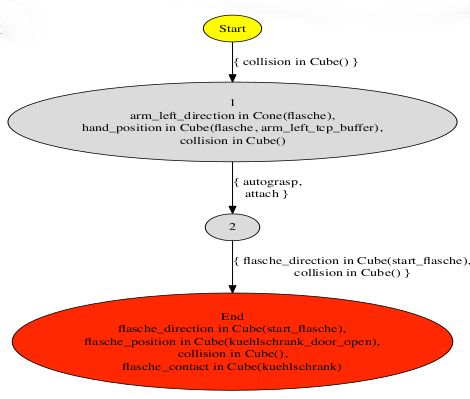
\includegraphics[width=0.6\linewidth]{figures/ch03_strategiegraph.png}
\caption{Beispiel eines Strategiegraphen: \Gu Einschenken\Go $\rightarrow$ Die Ausführungsumgebung bezieht sich auf Unterschiede in Objekten,
Objektposen und Hindernissen (verglichen mit Demonstrationen). Einschränkungen im Strategiegraphen referenzieren Koordinatensysteme. Deren Lage wird automatisch adaptiert. Bei Ausführung unter Verwendung von Bahnplanung repräsentieren die Knoten des Graphen Teilziele der Manipulationsaufgabe, seine Kanten Übergänge zwischen den Teilzielen. Ein Planungsproblems wird für jedes Teilziel gelöst.}
\label{fig:ch03_stratgra}
\end{figure}

\noindent
Im Folgenden soll der PdV-Zyklus (vgl. Abbildung \ref{fig:ch03_zykl}) beispielhaft an IPoR II 
verdeutlicht werden. %Hierzu viele potentiell relevante Bilder auf den Folien 
\paragraph*{Beobachtung} Als Sensorik wird verwendet: Mikrofon, Deckenkameras, Stereokamera mit Pan-Tilt-Unit, Flock-of-Birds, Voodoo, Cybergloves\\
Virtual Technology - Datenhandschuh, Meßprinzip: Dehnmessstreifen, 20 Fingerbeugungs- und Spreizwinkel + 2 Freiheitsgrade im Handgelenk\\
Bestimmung der Position und Orientierung der menschlichen Hände sowie von Objekten: Magnetfeldbasierter Positionstracker, Stereokamera

\paragraph*{Segmentierung}
\begin{itemize}
\item Ziel (mit Interpretationsphase): Repräsentation der demonstrierten Handlung durch Sequenz von zu
erfüllenden Teilzielen (= Topologie des Strategiegraphs)
\item Ansatz: schwellwertbasierte Segmentierung zur Bestimmung von markanten Zeitpunkten der Demonstration
\item Vorteile: einfache Interaktionsmöglichkeit während der Demonstration, einfache Korrektur von Hypothesen
\item Erzeugung eines Segmentierungspunkt, wenn Hand-, Fingergeschwindigkeit gering ist und mindestens ein Finger Objektkontakt % vgl Skript, IPor 1 !!
hat
\end{itemize}

\paragraph*{Interpretation} 
\begin{itemize}
\item Klassifikation der Segmentierungspunkte in 4 Typen auf Basis des Weltzustands an den Intervallgrenzen: 
\begin{itemize}
\item Kein Objekt
\item Objekt aufgenommen
\item Objekt gehalten
\item Objekt losgelassen
\end{itemize}
\item Lernen des Planungsmodells
\begin{itemize}
\item  Topologie des Strategiegraphs: Segmentierung der Bewegungen des linken und rechten Arms, Kombination zu einem Graphen (vgl. \autoref{sg})
\item Erzeugung der Bewegungseinschränkungen: Manuell definierte Koordinatensysteme für alle Objekte: $K = \{ \text{Flaschenöffnung, Becheröffnung,
Rechter Zeigefinger, Welt, ...} \}$; Erzeugung aller möglichen Einschränkungen $(t, f, M, g, R)$ mit $f,g \in K$, Typ $t$ beliebig,
für jeden Knoten und jede Kante $\rightarrow$ Region $R$ muss bestimmt werden (vgl. \autoref{sg1})
\item Beispiel: $f$ = Flaschenöffnung, $g$ = Welt, $t$ = Richtung; $f$ = Flaschenöffnung, $g$ = Becheröffnung, $t$ = Position
\end{itemize}
\begin{figure}[h!]
	\centering
	\begin{subfigure}{.4\textwidth}
		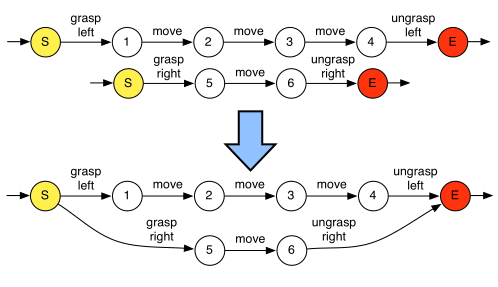
\includegraphics[width=\textwidth]{figures/ch03_stratgraph.png}
		\caption{}
		\label{sg}
	\end{subfigure}
	\begin{subfigure}{.4\textwidth}
		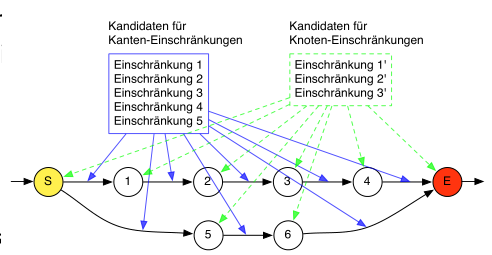
\includegraphics[width=\textwidth]{figures/ch03_stratgraph1.png}
		\caption{}
		\label{sg1}
	\end{subfigure}
	\caption{}
\end{figure}
\item Bestimmung der Region $R$: Für jede Einschränkung $(t, f, M, g, R)$
\begin{itemize}
\item Bestimmung des Werts von $f$ in jedem Punkt $t_i$ des Segments: $g^H_f(t_i) \cdot M$
\item Umwandlung in 3d-Vektor $m^\prime(t_i)$
\item Ergebnis: Menge von 3d-Vektoren
\item Bestimme Region $R$, die alle 3d-Vektoren einschließt
\ita Beispiel: Knoten-Einschränkung ($f$ = Flaschenöffnung, $g$ = Becheröffnung, $t$ = Position)
\end{itemize}
\end{itemize}
\paragraph*{Abstraktion}
Ziel: Anwendbarkeit des Planungsmodells in neuen Situationen auf verschiedenen Robotern
\begin{itemize}
\item Weitere Einschränkungen: Kräfte, Kontakte, Objektbewegung
\item Wesentliche Abstraktion durch Koordinatensysteme und Einschränkungen
\ita Abbildung von objektabhängigen Koordinatensystemen, \\z.B. Flasche.Öffnung $\rightarrow$ Milchpackung.Öffnung
\end{itemize} 

\paragraph*{Ausführung}
\begin{itemize}
\item Gelernte Einschränkungen definieren Suchraum für Roboterbewegungen
\item Einsatz von \textit{Bahnplanung unter Einschränkungen} zur Ausführung von gelernten
Planungsmodellen
\item Einsatz von \textit{Griffplanung} zur Bestimmung qualitativ hochwertiger Griffe
\end{itemize}
Eine Bewertung des Verfahrens ist in Tabelle \ref{tab:ipo} dargestellt.
\begin{table}[hbt]
\centering
\begin{tabular}{|p{6.5cm}|p{6.5cm}|}
\hline
Vorteile & Nachteile\\
\hline
\vspace{-5mm}
\begin{itemize}
\setlength\itemsep{0em}
\item[+] Generalisierung auf Basis von Objekteigenschaften
\item[+] Start- und Zielbeschreibung, Validierbarkeit
\item[+] Hindernisvermeidung und Berücksichtigung von Einschränkungen
\item[+] mehrere Lösungen und beliebige Optimalitätskriterien
\end{itemize}
 &
 \vspace{-5mm}
\begin{itemize}
\setlength\itemsep{0em}
\item[-] hoher Aufwand (Planungszeit, Simulationszeit)
\item[-] 3d-Modelle der Objekte, menschlichen Hand notwendig
\item[-] automatische Segmentierung bei dynamischen Bewegungen schwierig
\end{itemize}\\
\hline
\end{tabular}
\caption{Zusammenfassung: IPOR II}
\label{tab:ipo}
\end{table}\\ 
%Nächste VL:
%• Bahnplanung
%• Grifftaxonomie
%• Griffplanung


%Übung I (5. VL)
\section{Aktionsplanungsverfahren} %(6. VL)
\section{Probabilistisches Entscheiden} %(7.-9. VL)
%Übung II (10. VL)
%Stand der Technik bei Autonomen Roboterassistenten (11. VL) -> nicht behandelt



\end{document}


%%% Local Variables:
%%% mode: latex
%%% TeX-master: t
%%% End: